
\chapter{Experimental Evaluation}
\label{ch:eval}

\section{Data Exploration}
\subsection{Adult Dataset}
\label{sec:adult}

\begin{itemize}
    \item Age: The age of the individual (Positive integer)
    \item Work class: The sector the individual works in (8 Categories)
    \item fnlgwgt: A weight determined by the census bureau (Positive integer)
    \item Education: Highest educational degree (16 categories)
    \item Educaitional-num: Enumerated education (16 categories)
    \item Marital Status: Marital status of individual (7 Categories)
    \item Occupation: General type of occupation (15 categories)
    \item Relationship: What kind of relationship the individual is to others (6 categories)
    \item Race: What race the individual belongs to (6 Categories)
    \item Gender: Biological sex of the individual (2 Categories)
    \item Capital gain: Capital gain of individual (Positive integer)
    \item Capital loss: Capital loss of the individual (Positive integer)
    \item Native country: Native country of the individual (42 categories)
    \item Income: Whether individual makes more than 50K or not (2 Categories)
\end{itemize}

This dataset consists of mostly categorical attributes which are not ordinal. This makes analysis quite challenging. Many models assume Gaussian distributions, which is not present in the dataset. In this dataset, there are also some sensitive attributes, most notably \emph{Gender} and \emph{Race}. One could also argue that \emph{Marital Status} and \emph{Relationship} could also be sensitive attributes.

In a fair machine learning system, we would expect that the outcome in terms of income does not depend on the race, gender, marital status or relationship or the very least that the decision by the model is independent of the sensitive attributes.

\subsection{Attributes correlated with income}

\begin{table}
    \centering
    \begin{tabular}{lr}
        \toprule
        Attribute &  Correlation \\
        \midrule
        marital-status.Never-married &    -0.318782 \\
        relationship.Own-child       &    -0.225691 \\
        relationship.Not-in-family   &    -0.190372 \\
        occupation.Other-service     &    -0.155254 \\
        relationship.Unmarried       &    -0.143642 \\
        education.HS-grad            &    -0.130706 \\
        race.Black                   &    -0.090448 \\
        education.11th               &    -0.086728 \\
        occupation.Adm-clerical      &    -0.086475 \\
        relationship.Other-relative  &    -0.085601 \\
        \bottomrule
    \end{tabular}
    \caption{Features that are negatively correlated with income.}
    \label{fig:negative_income_correaltion}
\end{table}

\begin{table}
    \centering
    \begin{tabular}{lr}
        \toprule
        Attribute &  Correlation \\
        \midrule
        education.Masters                 &     0.174184 \\
        education.Bachelors               &     0.180371 \\
        occupation.Prof-specialty         &     0.188793 \\
        occupation.Exec-managerial        &     0.210938 \\
        gender.Male                       &     0.214628 \\
        capital-gain                      &     0.223013 \\
        hours-per-week                    &     0.227687 \\
        age                               &     0.230369 \\
        marital-status.Married-civ-spouse &     0.445853 \\
        \bottomrule
    \end{tabular}
    \caption{Features that are positively correlated with income.}
    \label{fig:positive_income_correaltion}
\end{table}

We see  in that there are some categories in the following attributes that are correlated with income

\begin{itemize}
    \item Marital Status
    \item Age
    \item Hours per week
    \item Capital Gain
    \item Occupation
    \item Relationship
    \item Education
    \item Gender
    \item Race
\end{itemize}

We observe that our identified sensitive attributes are correlated with income. The challenge now is that we have to learn a model that does not treat individuals belonging to different classes in the sensitive attribute unfairly.

\section{Experiment 1: FairBN, FairTreeClassifier vs NB}


\label{sec:result:experiment1}

Below we will go through the different results of the first round of experiments. To see the detailed results, these are available in the appendix. See~\ref{app:experiment1}

\begin{figure}
    \centering
    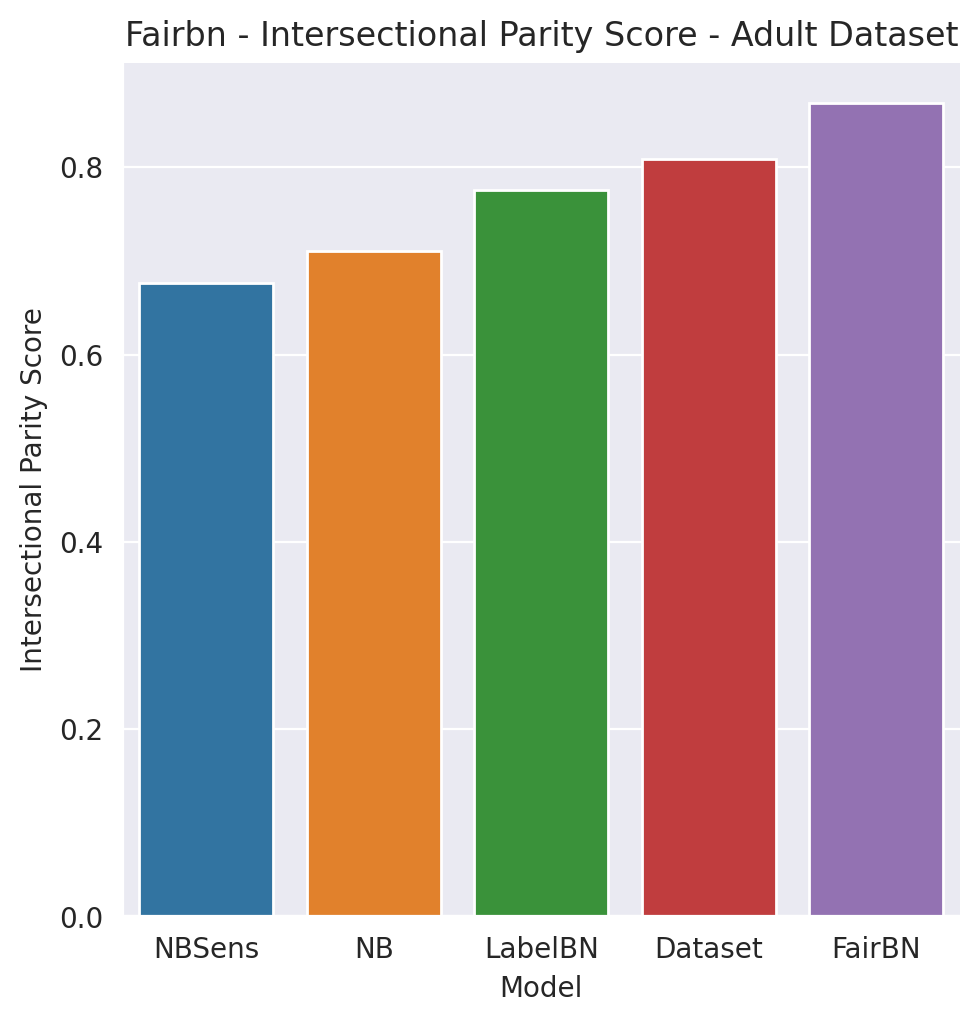
\includegraphics[width=0.49\linewidth]{figures/adult_fairbn_parity.png}
    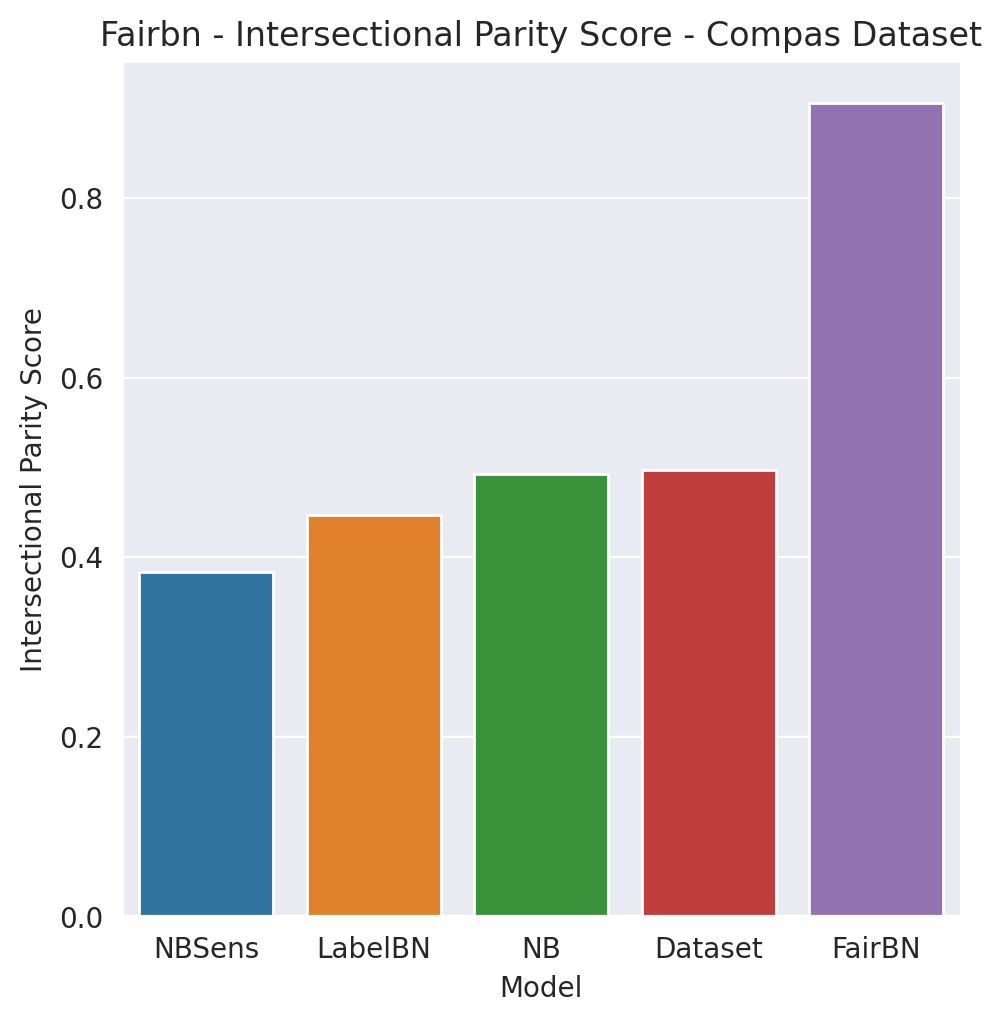
\includegraphics[width=0.49\linewidth]{figures/compas_fairbn_parity.png}
    \caption{Intersectional Parity Score for fair Bayesian network vs naïve bays.}
    \label{fig:exp1fairBNparity}
\end{figure}

\subsection{Fair Bayesian Network}

After training the fair Bayesian network classifier on the adult and Compas dataset, we get an intersectional parity score of $0.87$ and $0.91$ respectively. This is better than the inherent parity score in the dataset labels, which is $0.81$ and $0.51$ respectively. These results and how the different methods compare to one another is shown in figure~\ref{fig:exp1fairBNparity}.

In terms of accuracy and traditional performance of the model, we observe that there is a tradeoff between performance and fairness. This is best shown in the ROC curve shown in figure~\ref{fig:exp1fairBNROC}. There is a slight drop in the fair Bayesian network compared to the naïve Bayes method.

We also observe a quite significant performance difference between the adult dataset and the Compas dataset. Why this is is not explored further in this thesis, as we are interested in seeing differences in performance with respect to fairness.  
\begin{figure}
    \centering
    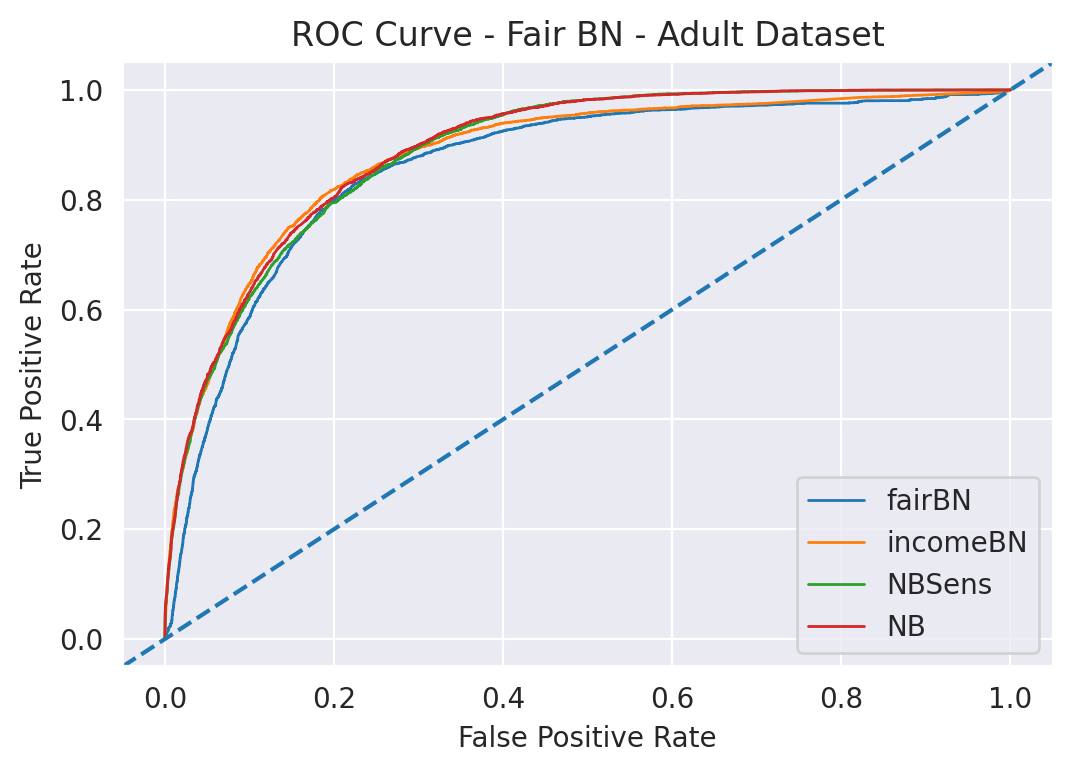
\includegraphics[width=0.49\linewidth]{figures/adult_fairbn_roc.png}
    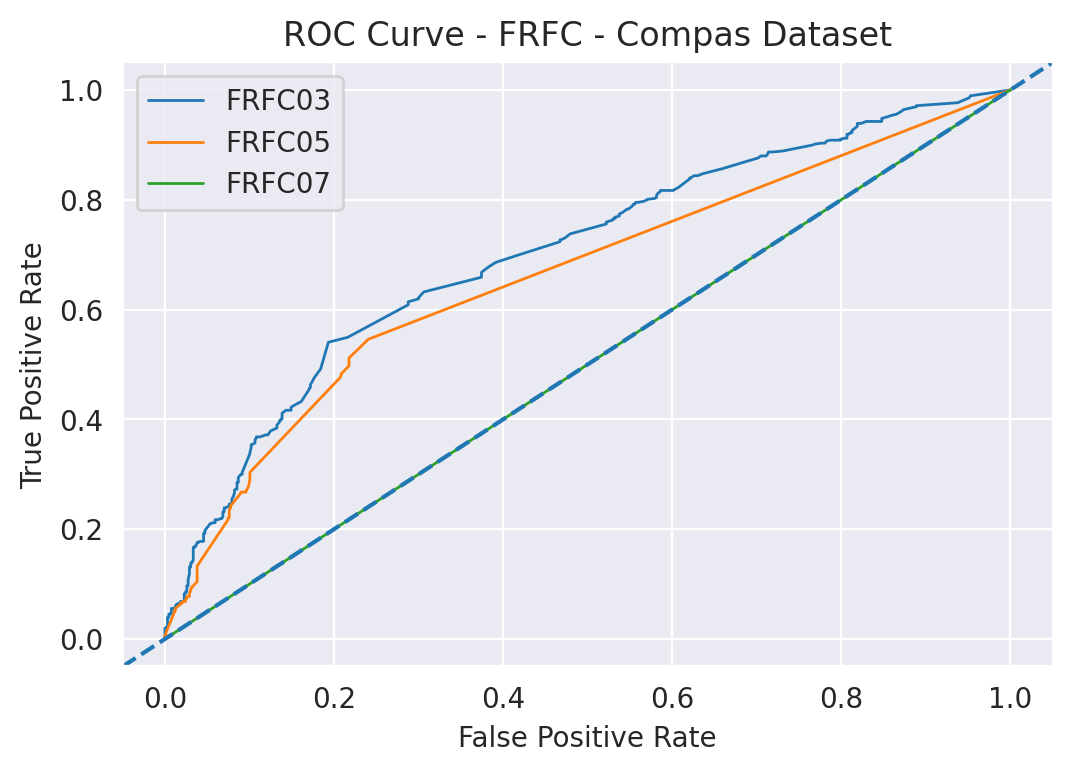
\includegraphics[width=0.49\linewidth]{figures/compas_frfc_roc.png}
    \caption{ROC curve for fair Bayesian network vs naïve Bayes.}
    \label{fig:exp1fairBNROC}
\end{figure}

\subsection{Fair Random Forest Classifier}

We ran the same experiments using their classifier on the adult dataset and Compas dataset. Rather interestingly, we do not observe any improvement in intersectional parity in the adult dataset for any of the methods, with the inherent intersectional parity for the dataset being $0.810$ and the best fair random forest classifier with $\Theta = 0.3$ having an intersectional parity of $0.78$, which is counterintuitive to the claimed meaning behind the hyperparameter $\Theta$ stated by the authors.

\begin{figure}
    \centering
    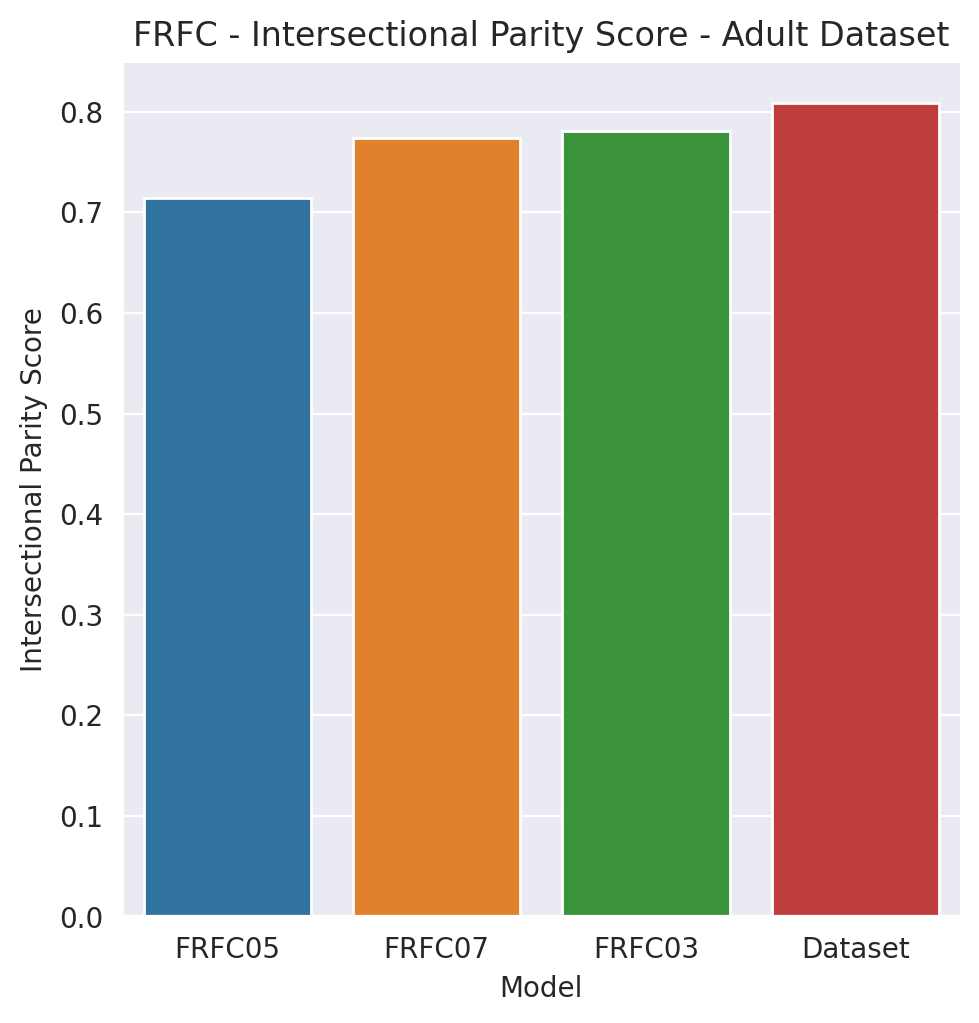
\includegraphics[width=0.49\linewidth]{figures/adult_frfc_parity.png}
    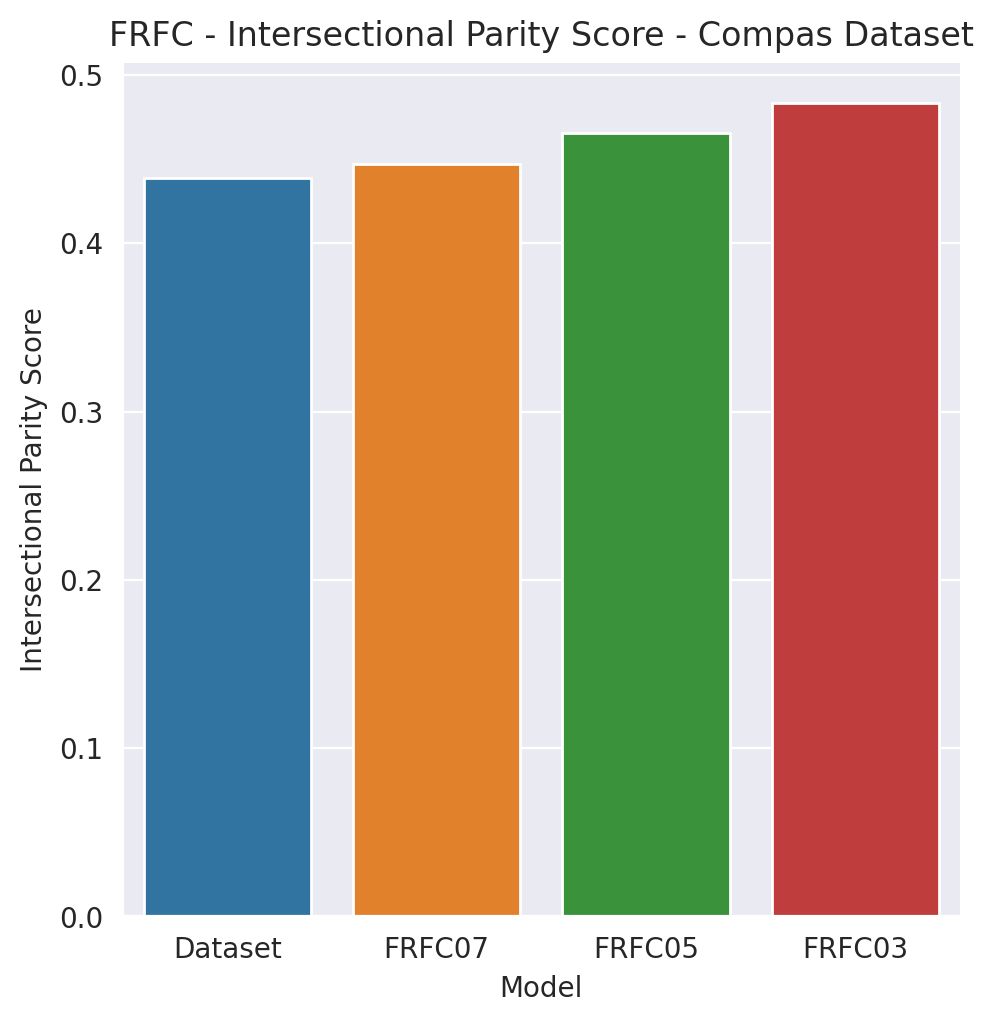
\includegraphics[width=0.49\linewidth]{figures/compas_frfc_parity.png}
    \caption{Parity score for fair random forest classifier.}
    \label{fig:exp1FRFCparity}
\end{figure}

For the Compas dataset, things are looking better with the models with $\Theta \in \{0.3, 0.7\}$ having higher intersectional parity scores than is inherent in the dataset labels. Still, the results given the stated meaning behind $\Theta$ is counterintuitive. The parity scores are shown in figure~\ref{fig:exp1FRFCparity}. The ROC curve for the different datasets is shown in figure~\ref{fig:exp1FRFCROC}

\begin{figure}
    \centering
    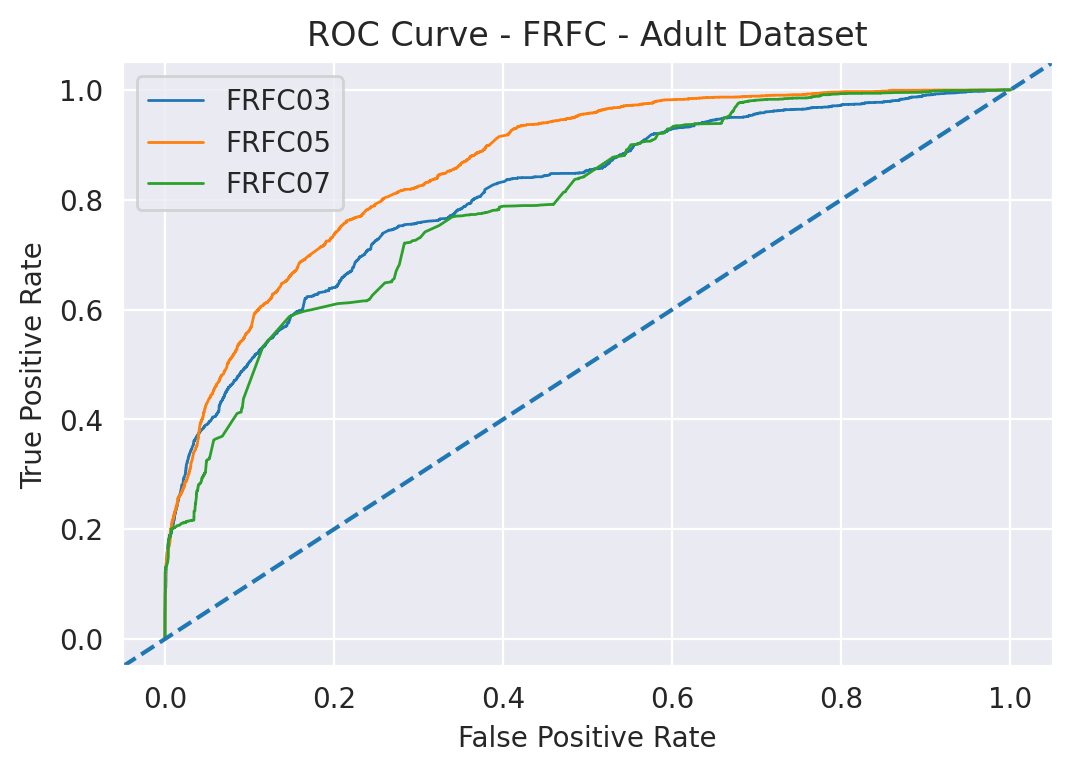
\includegraphics[width=0.49\linewidth]{figures/adult_frfc_roc.png}
    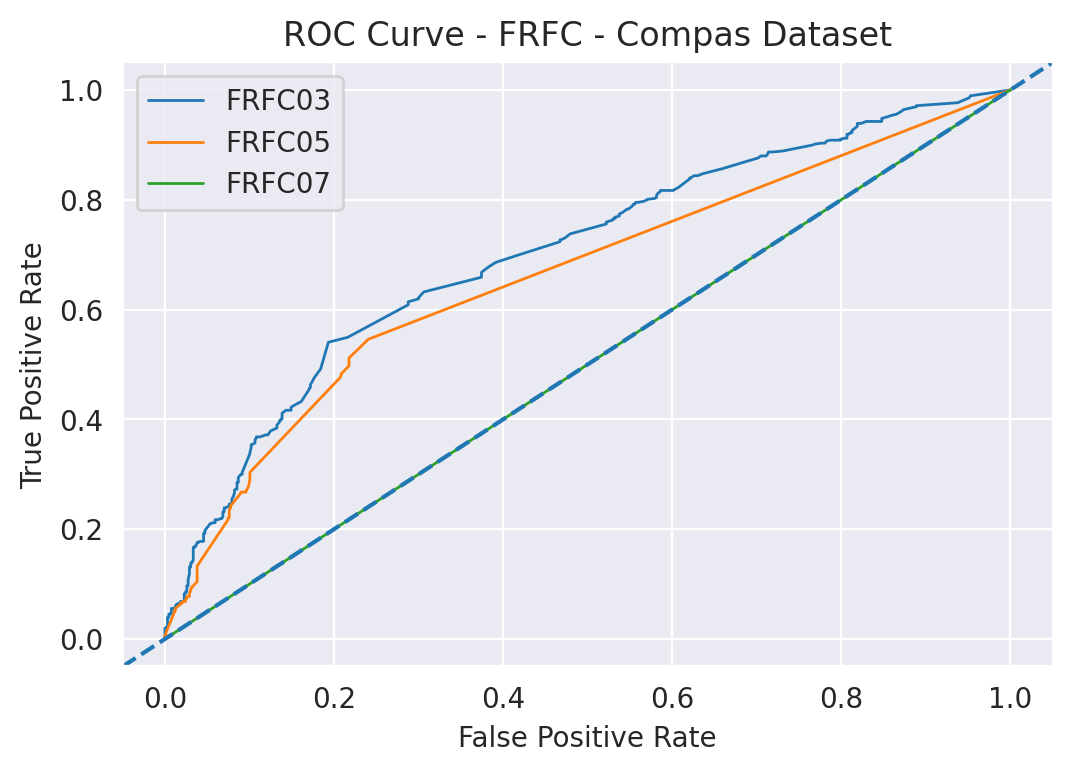
\includegraphics[width=0.49\linewidth]{figures/compas_frfc_roc.png}
    \caption{ROC curve for fair random forest classifier.}
    \label{fig:exp1FRFCROC}
\end{figure}

\section{Experiment 2: Results}
\label{eval:exp2}

\subsection{F1 Score}

\begin{figure}
    \centering
    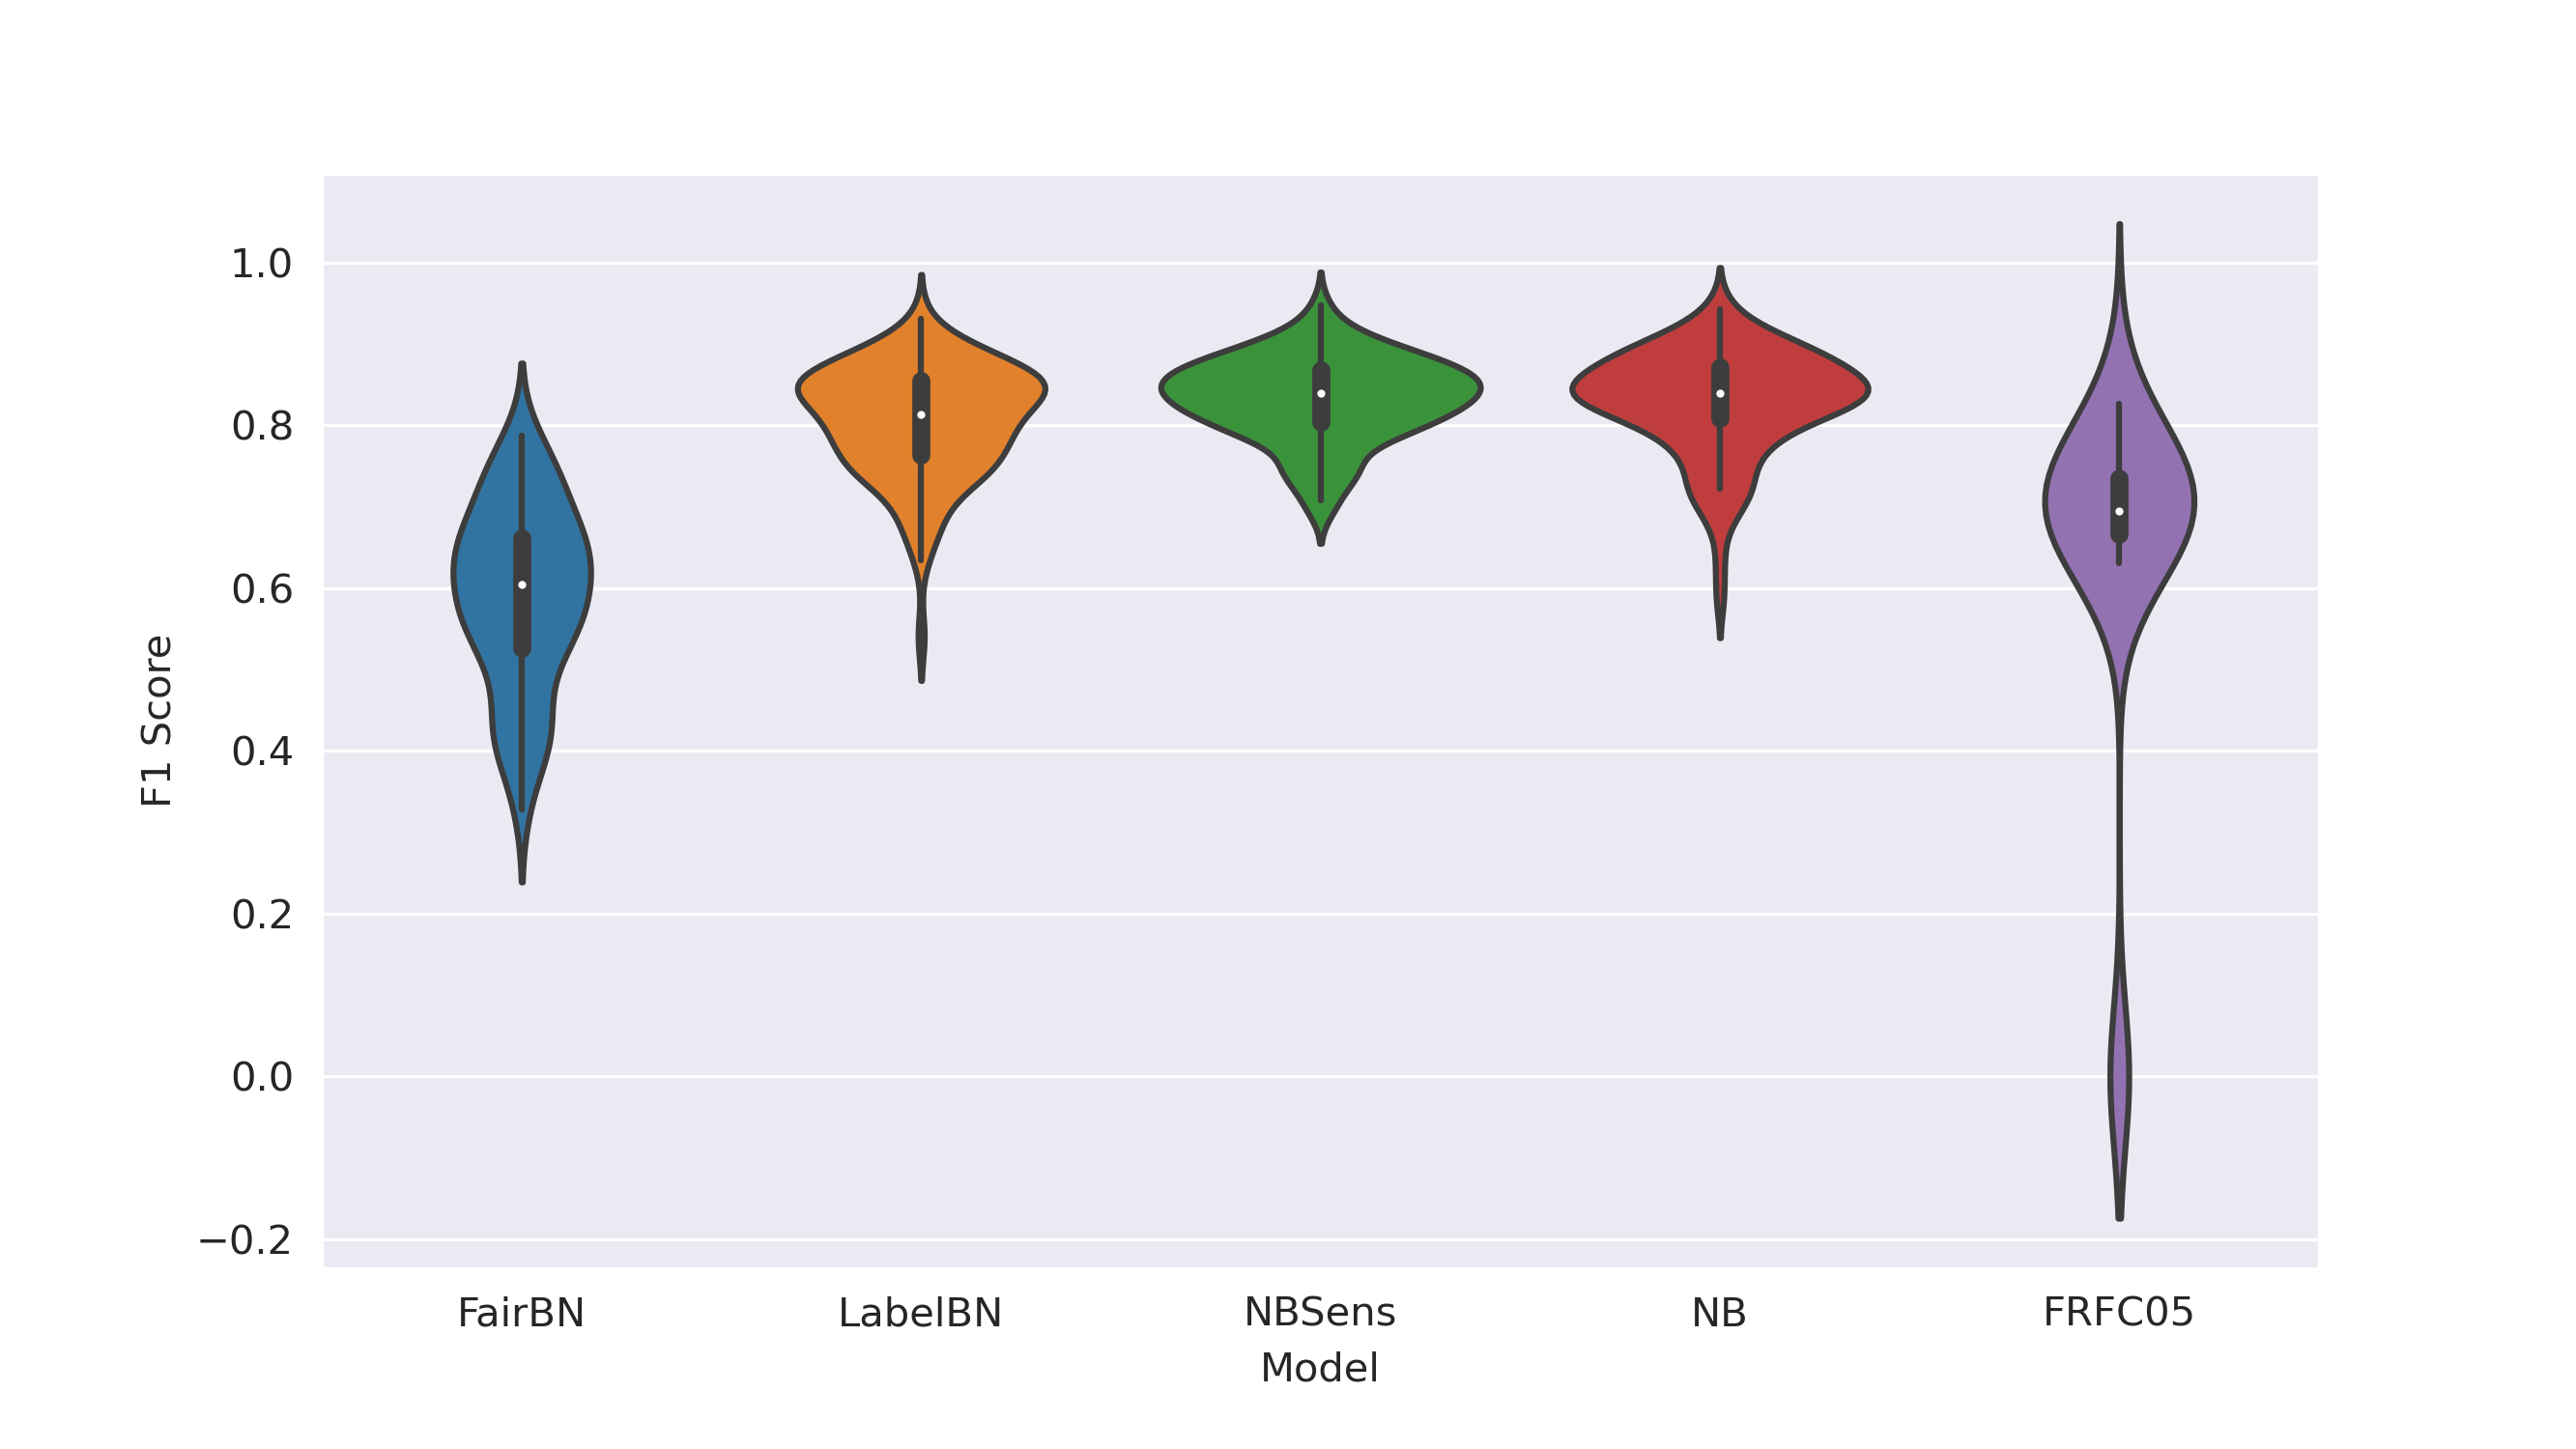
\includegraphics[width=\linewidth]{figures/F1score-synthethic.png}
    \caption{F1 Scores of the different models on 100 synthetic datasets. Higher is better.}
    \label{fig:f1synth}
\end{figure}

When evaluating the models in terms of F1 Score, we observe that the fair methods have lower but acceptable F1 Scores. For the fair Bayesian network classifier $95\%$ of the F1 scores is at $0.4$ or higher with mean at $0.6$. For the fair random forest classifier, these values are $0.0$ and $0.63$. We see from the plot in figure~\ref{fig:f1synth} that the F1 score of the fair Bayesian network is on average lower than for fair random forest classifier but with lower variance.

\subsection{Specificity}

\begin{figure}
    \centering
    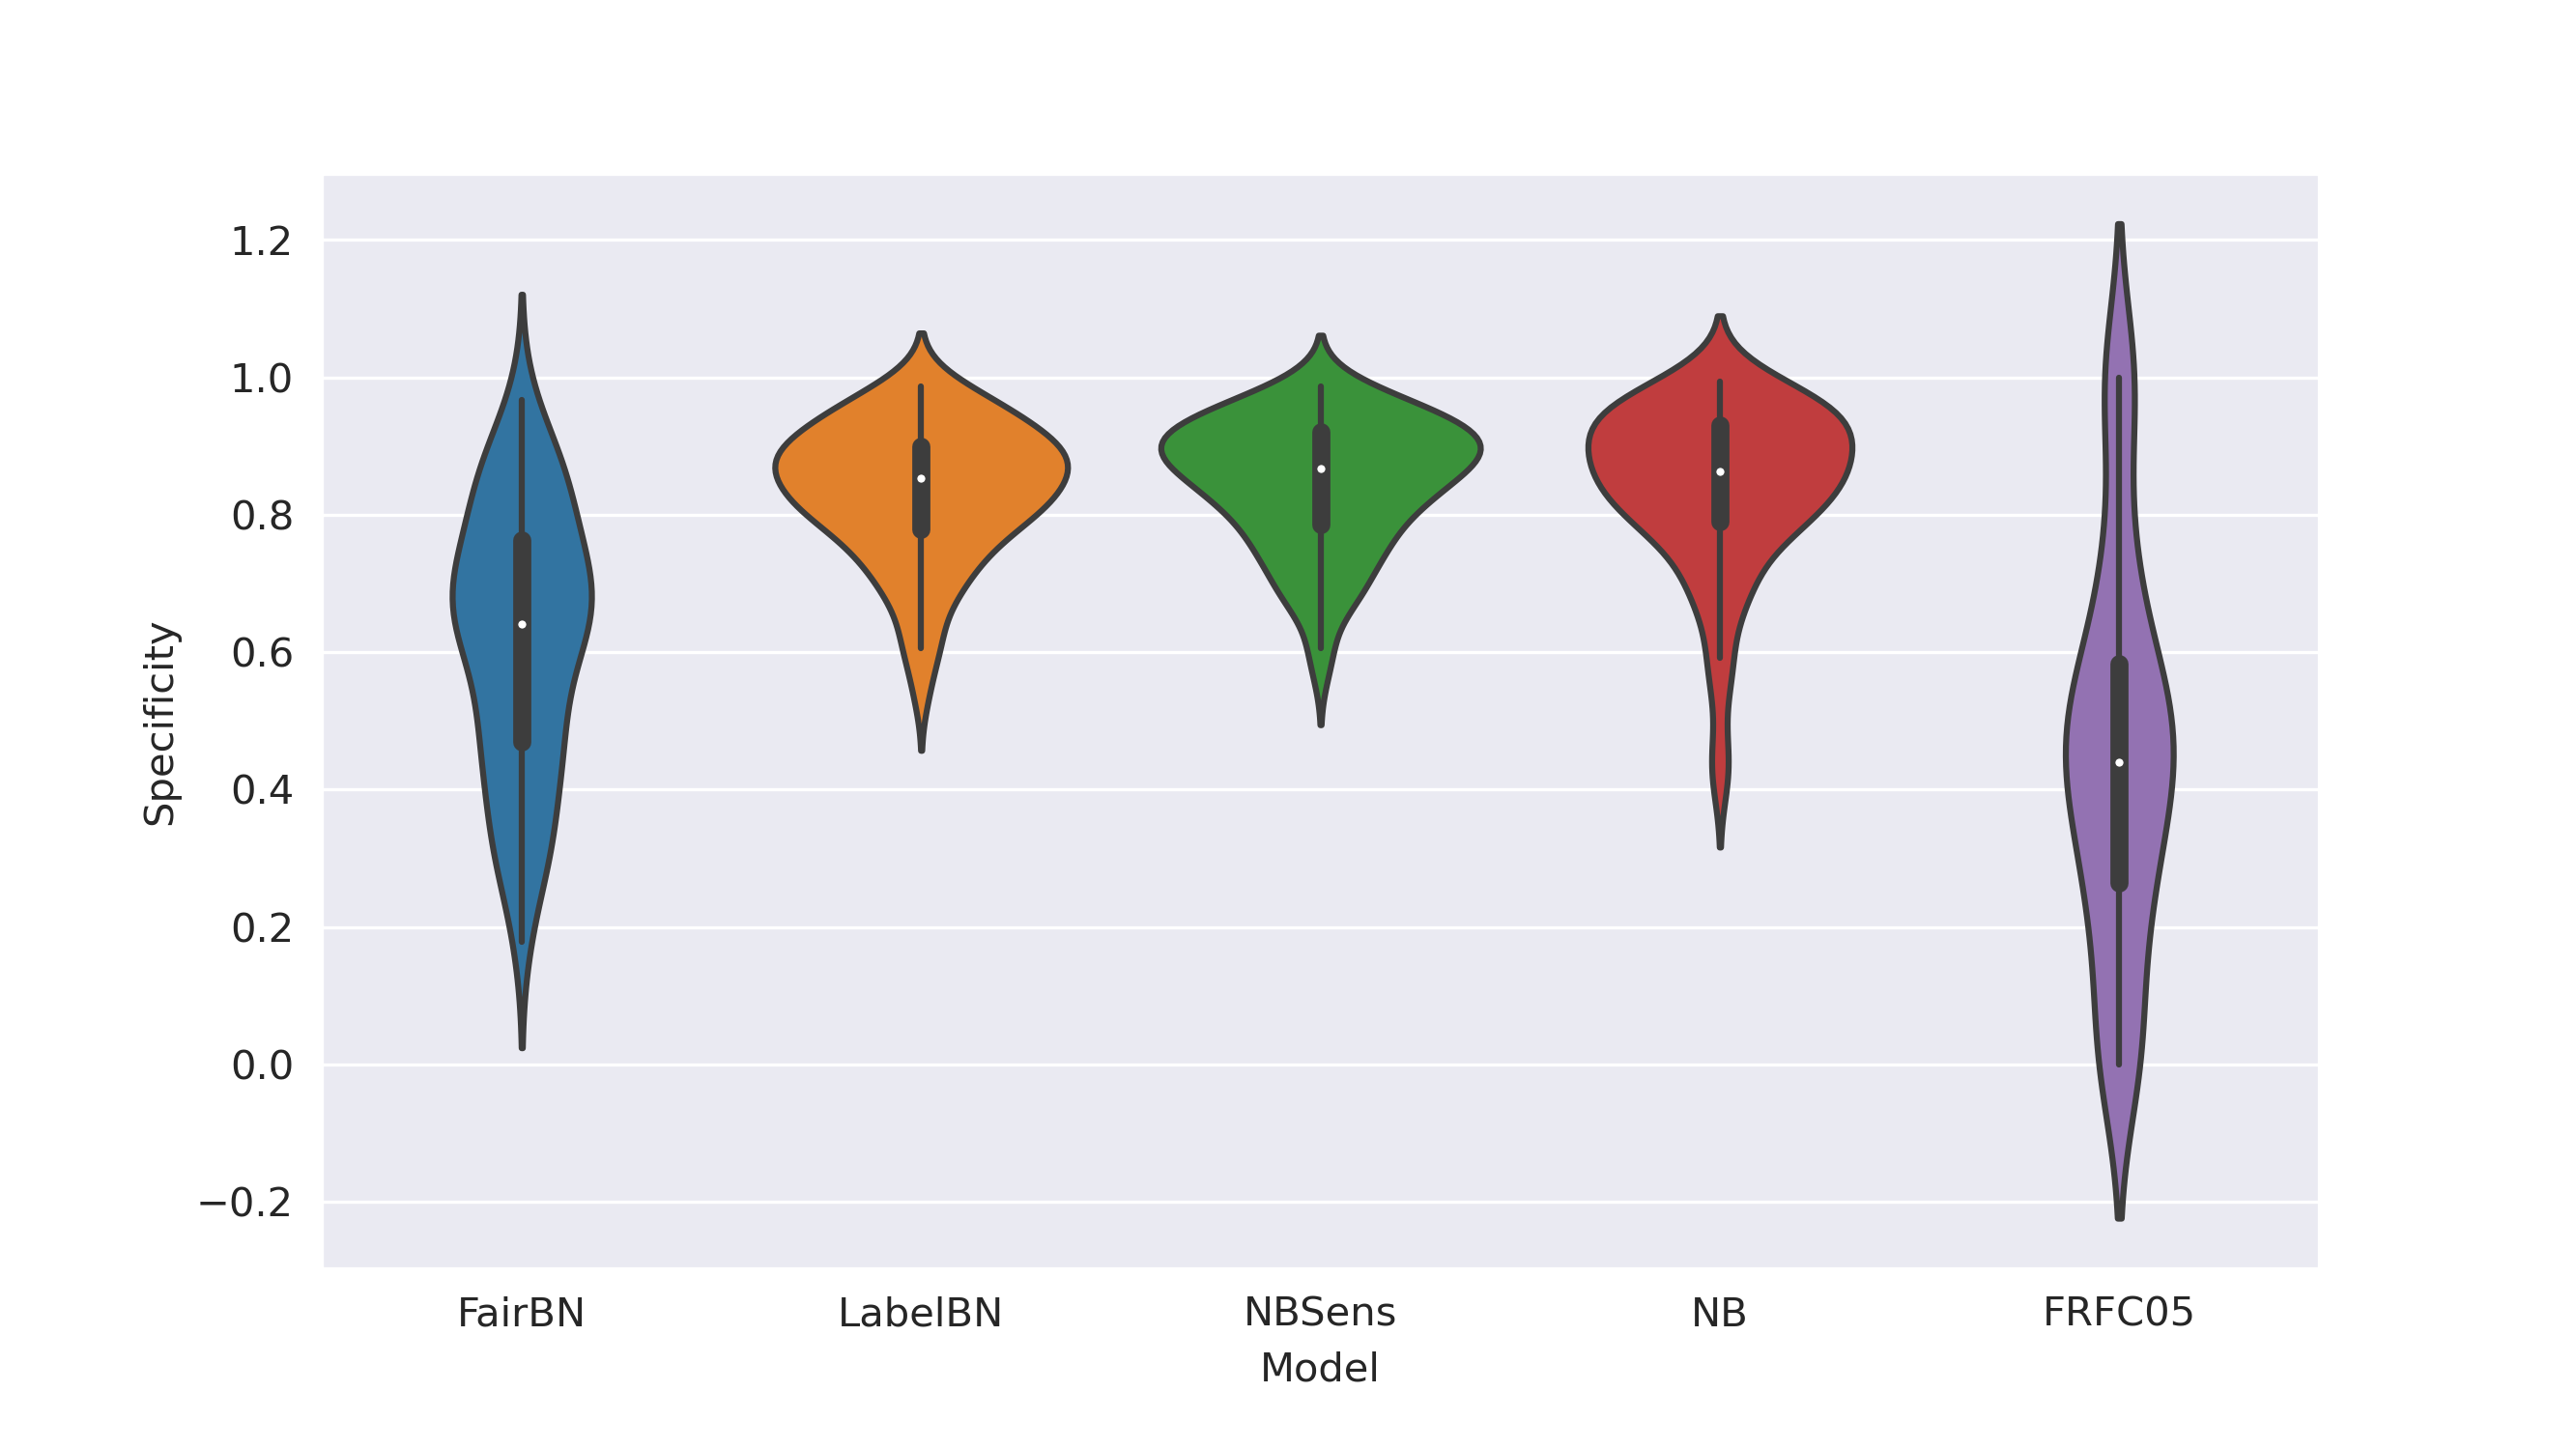
\includegraphics[width=\linewidth]{figures/Specificity-synthetic.png}
    \caption{Specificity of the different models on 100 synthetic datasets. Higher is better}
    \label{fig:specsynth}
\end{figure}

Since F1 Score is biased with respect to true negatives, we calculate the Specificity of the models as well. The distribution of specificity for the different models are shown in figure~\ref{fig:specsynth}. We observe that the fair methods has a higher variance in their specificity as compared to the naïve Bayesian methods as well as the unfair predictions of the fair Bayesian network. $95\%$ of the specificity values are at $0.3$ or higher with mean at $0.61$. For fair random forest classifier, these values are $0.0$ and $0.44$ respectively.

\subsection{Intersectional parity score}

\begin{figure}
    \centering
    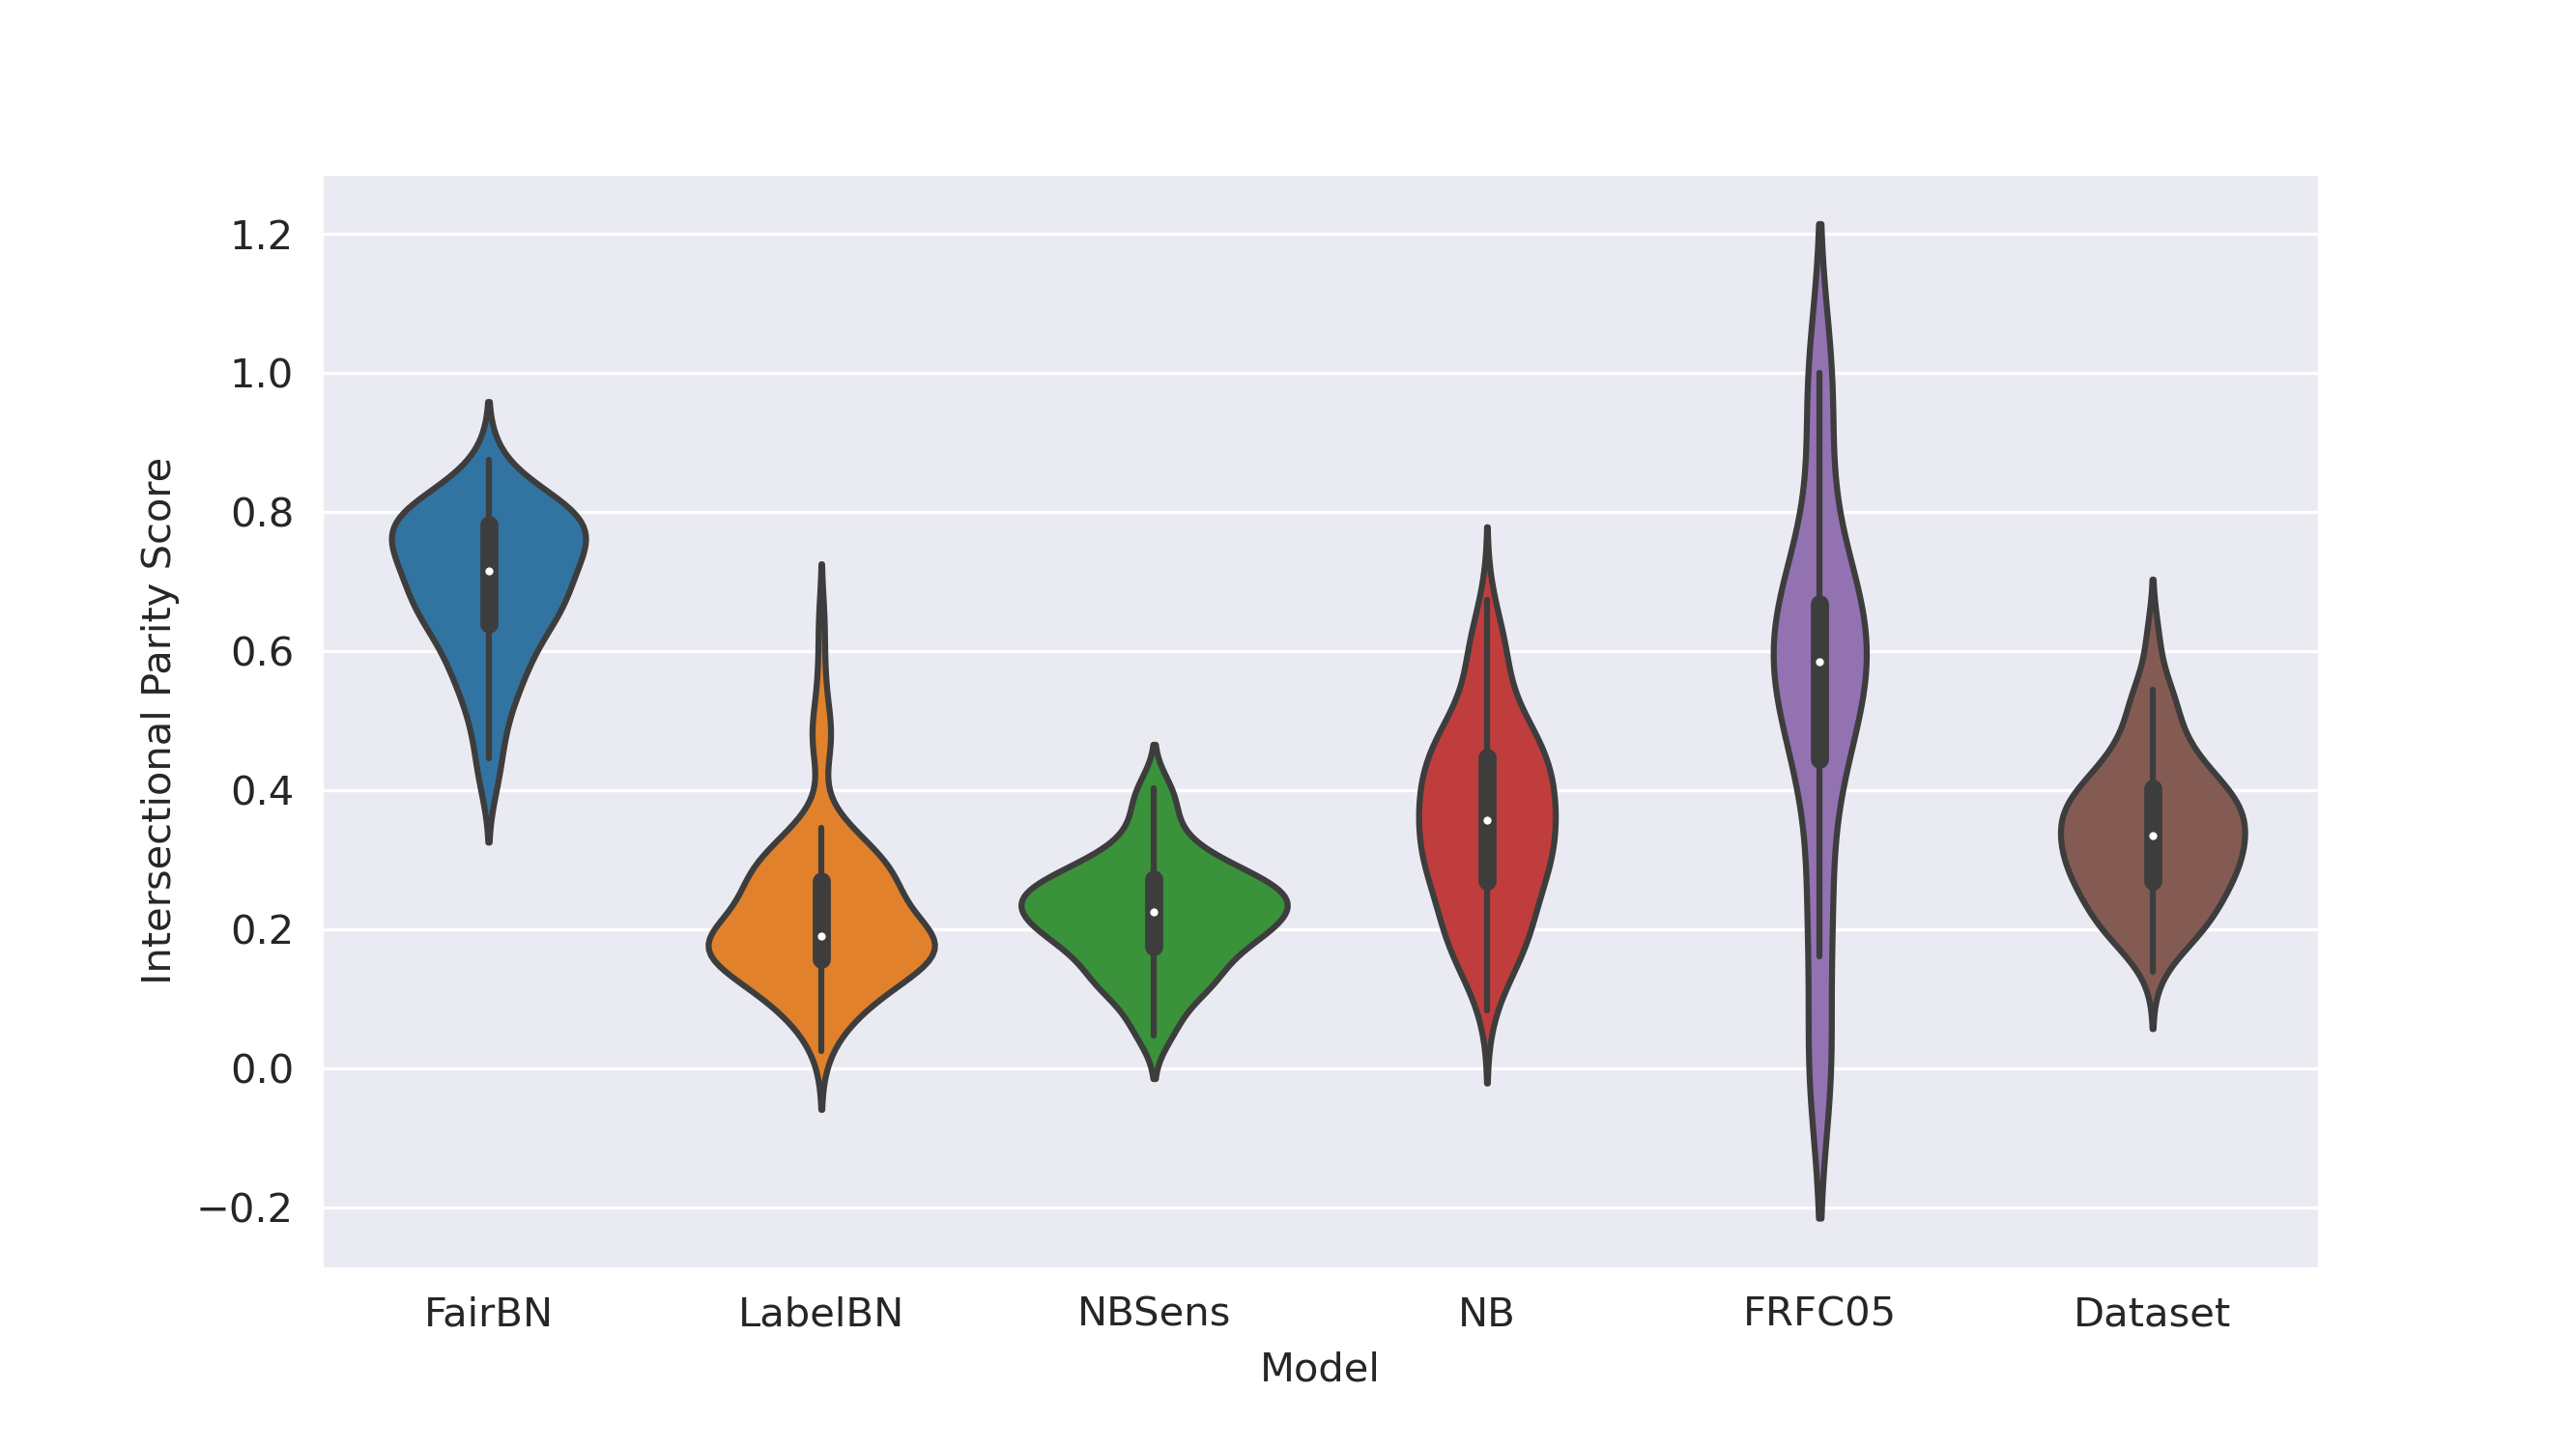
\includegraphics[width=\linewidth]{figures/intparscore-synthetic.png}
    \caption{Intersectional Parity Score of the different models on 100 synthetic datasets. Higher is better.}
    \label{fig:intpar}
\end{figure}

In terms of intersectional parity score, i.e. average demographic parity across all subgroups of sensitive attributes, we see that the fair Bayesian network is able to consistently have more fair decisions. See figure~\ref{fig:intpar}. The mean parity score for the FairBN classifier is $0.70$ with the 5th percentile at $0.50$. For the fair random forest classifier these values are $0.54$ and $0.0$ respectively.
 
\subsection{AUC Gender}

\begin{figure}
    \centering
    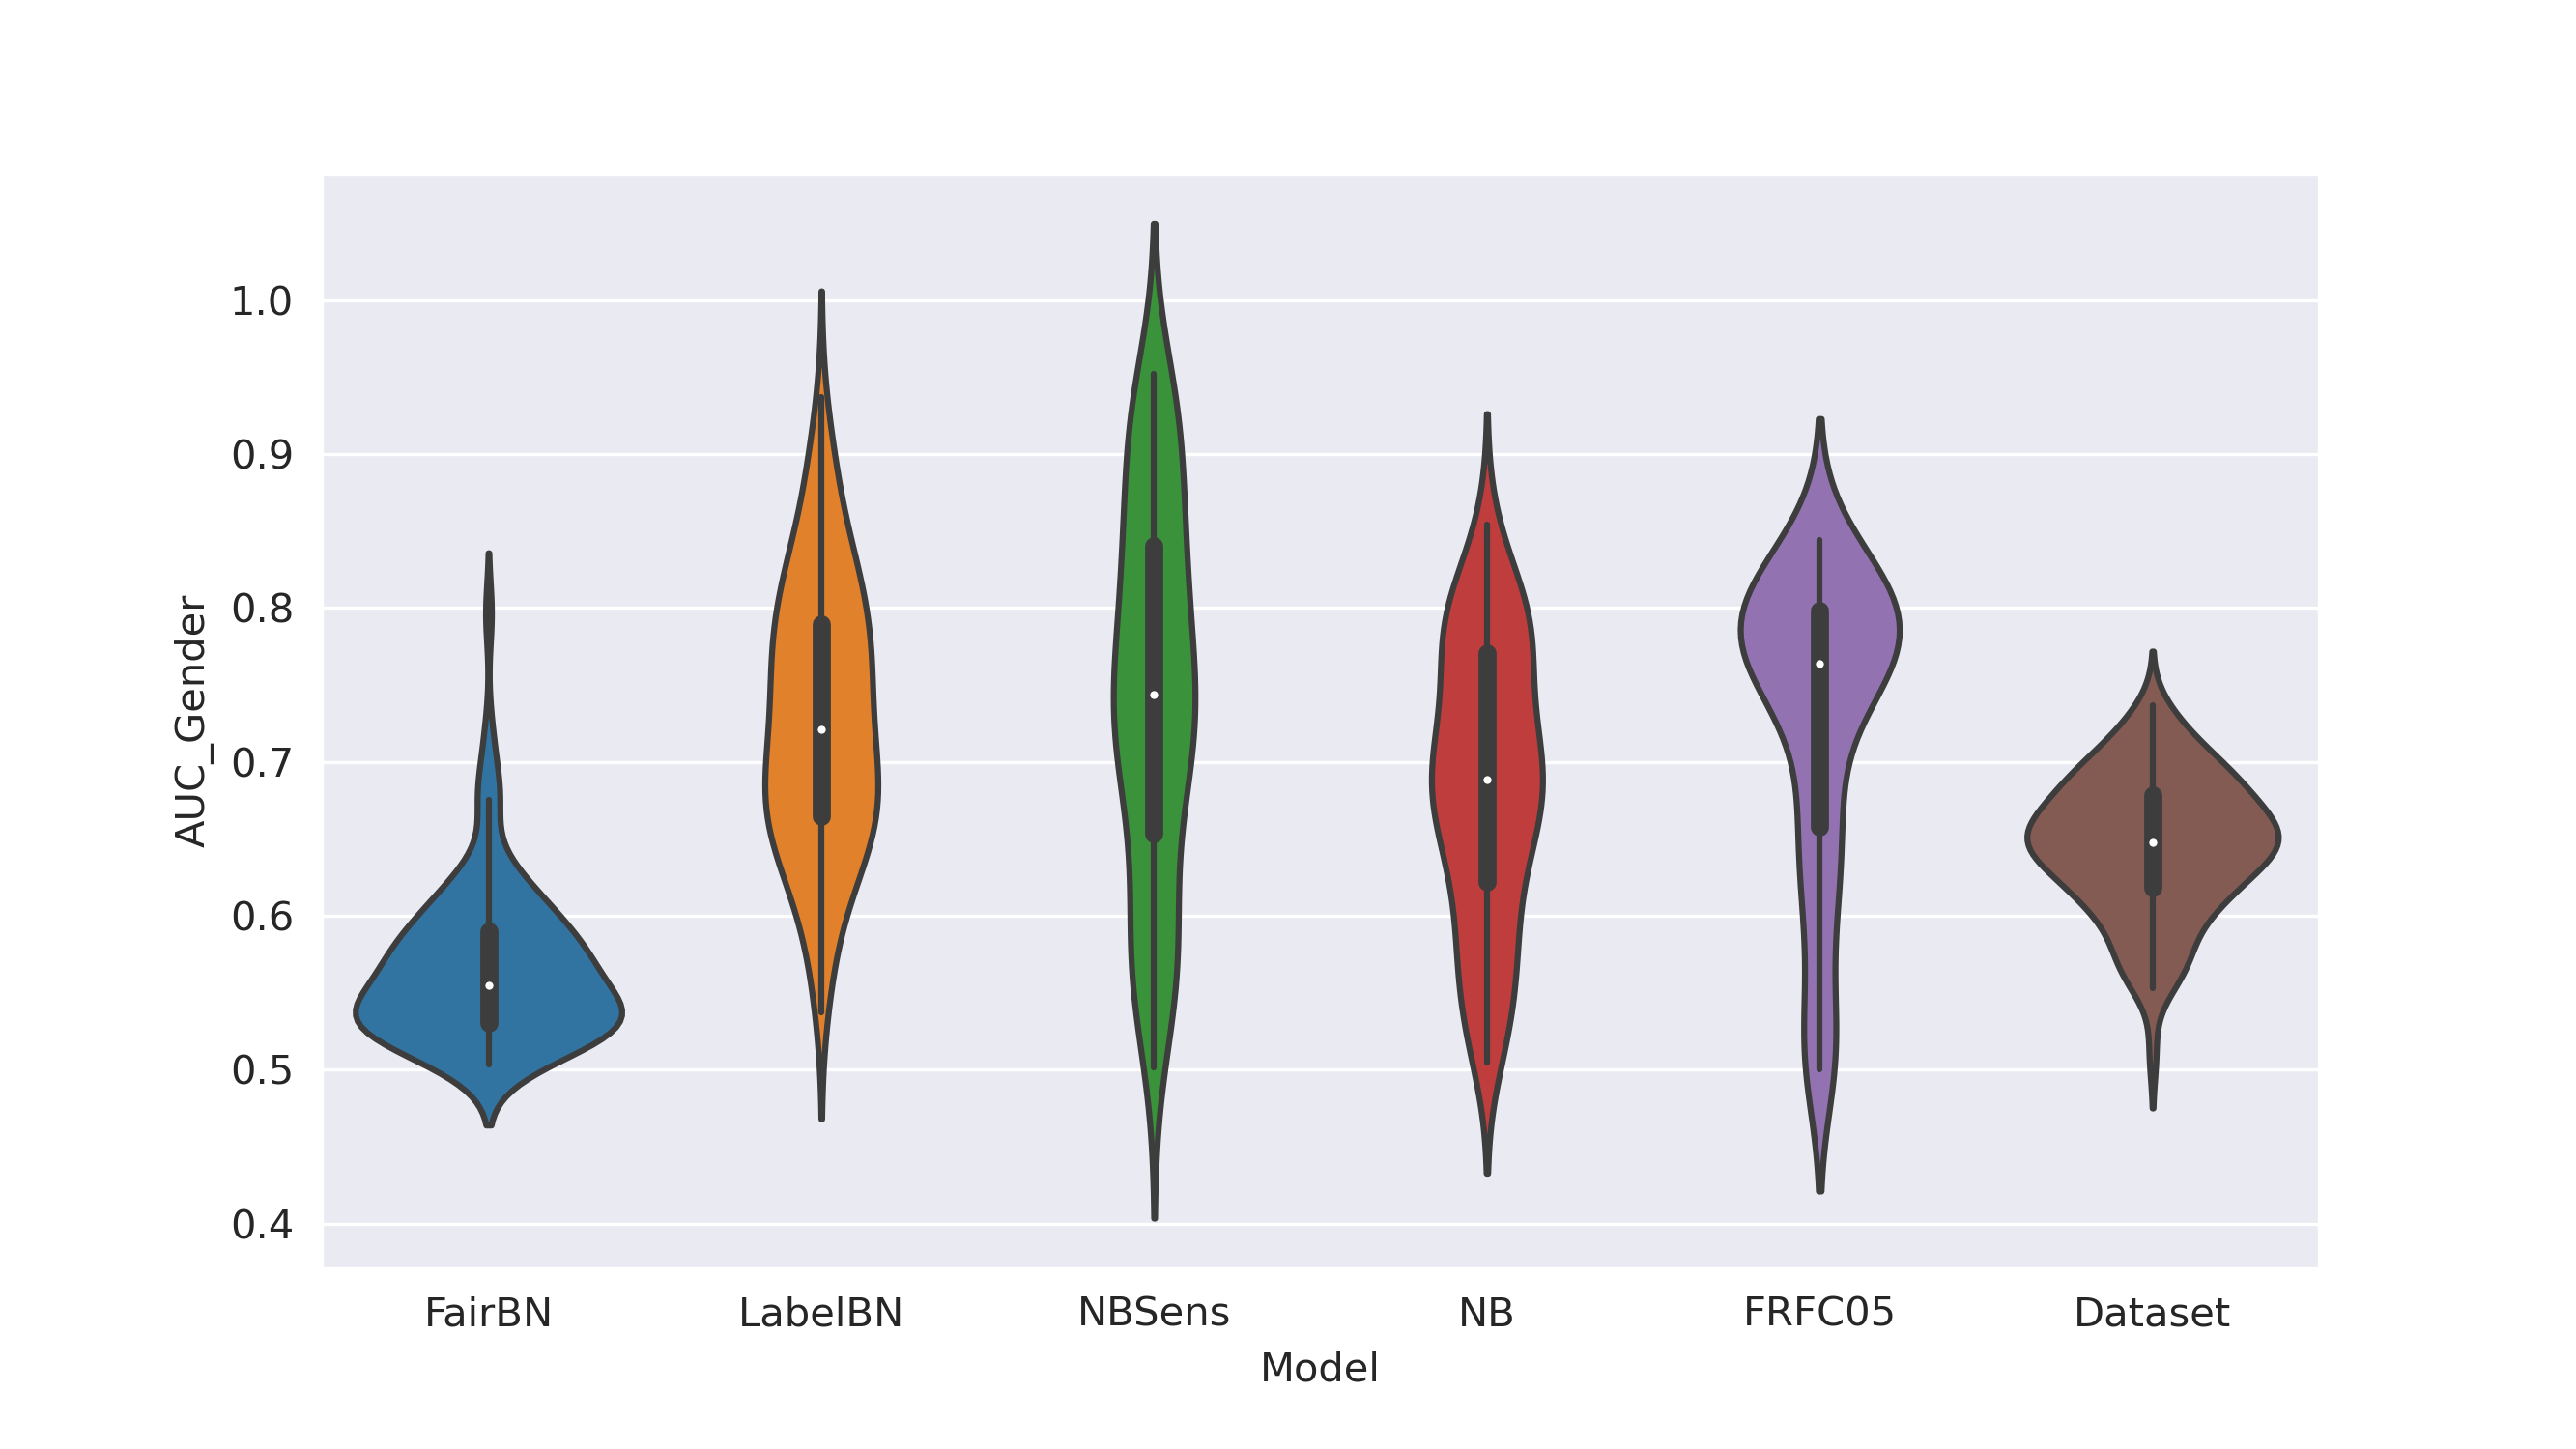
\includegraphics[width=\linewidth]{figures/aucg-synthetic.png}
    \caption{AUC w.r.t. Gender of the different models on 100 synthetic datasets. Lower is better.}
    \label{fig:aucgender}
\end{figure}

In the paper by \citet{Antonio:2021:arXiv} they propose use AUC w.r.t. gender to evaluate splits which are more fair. Interestingly, while the fair random forest method is based on selecting splits that minimise the AUC w.r.t. gender, the model fares quite similarly to the Naïve Bayes models and LabelBN. See figure~\ref{fig:aucgender} The AUC is even higher than what is inherent in the labels of the dataset itself and predictions are in this sense more discriminatory than what is present in the true labels. The only model to minimise AUC more than the inherent dataset labels is FairBN. FairBN has a mean AUC of $0.56$ and a 5th percentile of $0.51$. While for the fair random forest classifier, these values are $0.72$ and $0.51$ respectively.

\subsection{Kullback-Leibler Divergence}

\begin{figure}
    \centering
    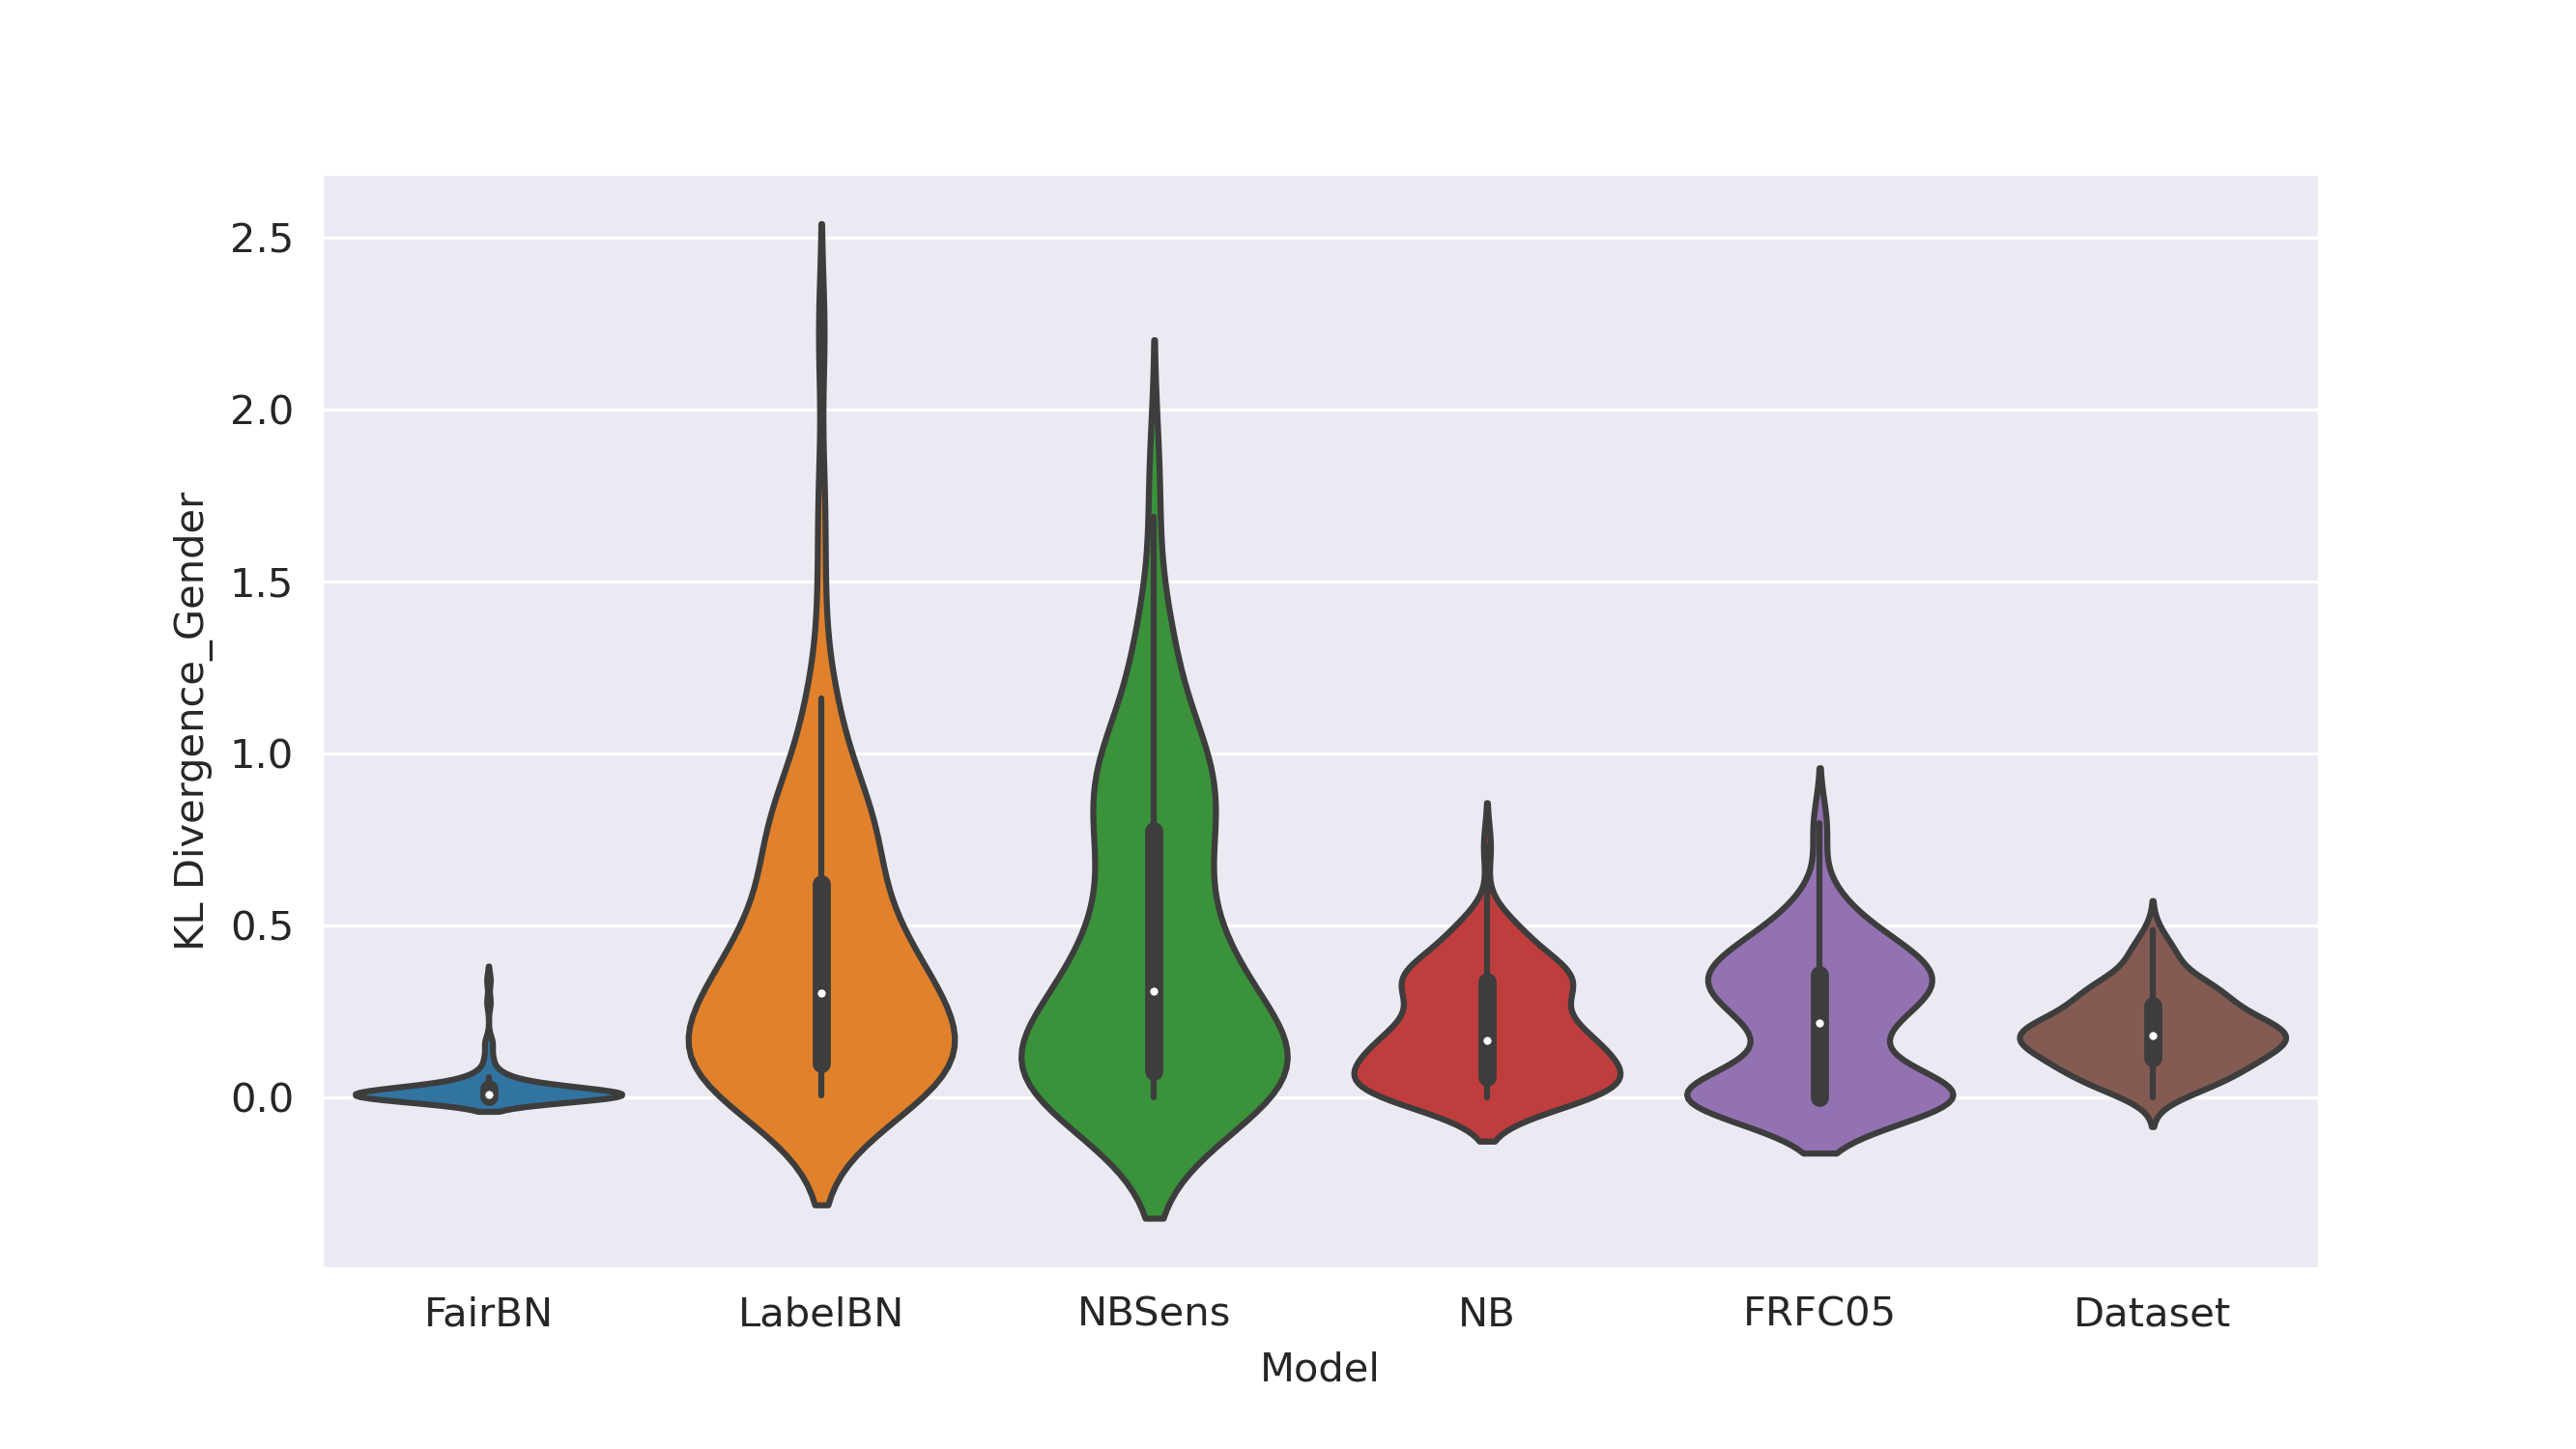
\includegraphics[width=\linewidth]{figures/kldg-synthetic.png}
    \caption{Kullback-Leibler Divergence of the different models on 100 synthetic datasets. Lower is better.}
    \label{fig:kldg-synthetic}
\end{figure}

Lastly, we evaluate the models in terms of Kullback-Leibler Divergence. Here we see a significant difference between the methods. See figure~\ref{fig:kldg-synthetic}The best performing model here is FairBN. With a 5th percentile value of $4.67 \times 10^{-5}$ and mean $0.025$. For the fair random forest classifier this is $0$ and $0.21$ respectively

\subsection{Correlation between scoring methods}

\subsubsection{Demographic Parity v KL Divergence}

\begin{figure}
    \centering
    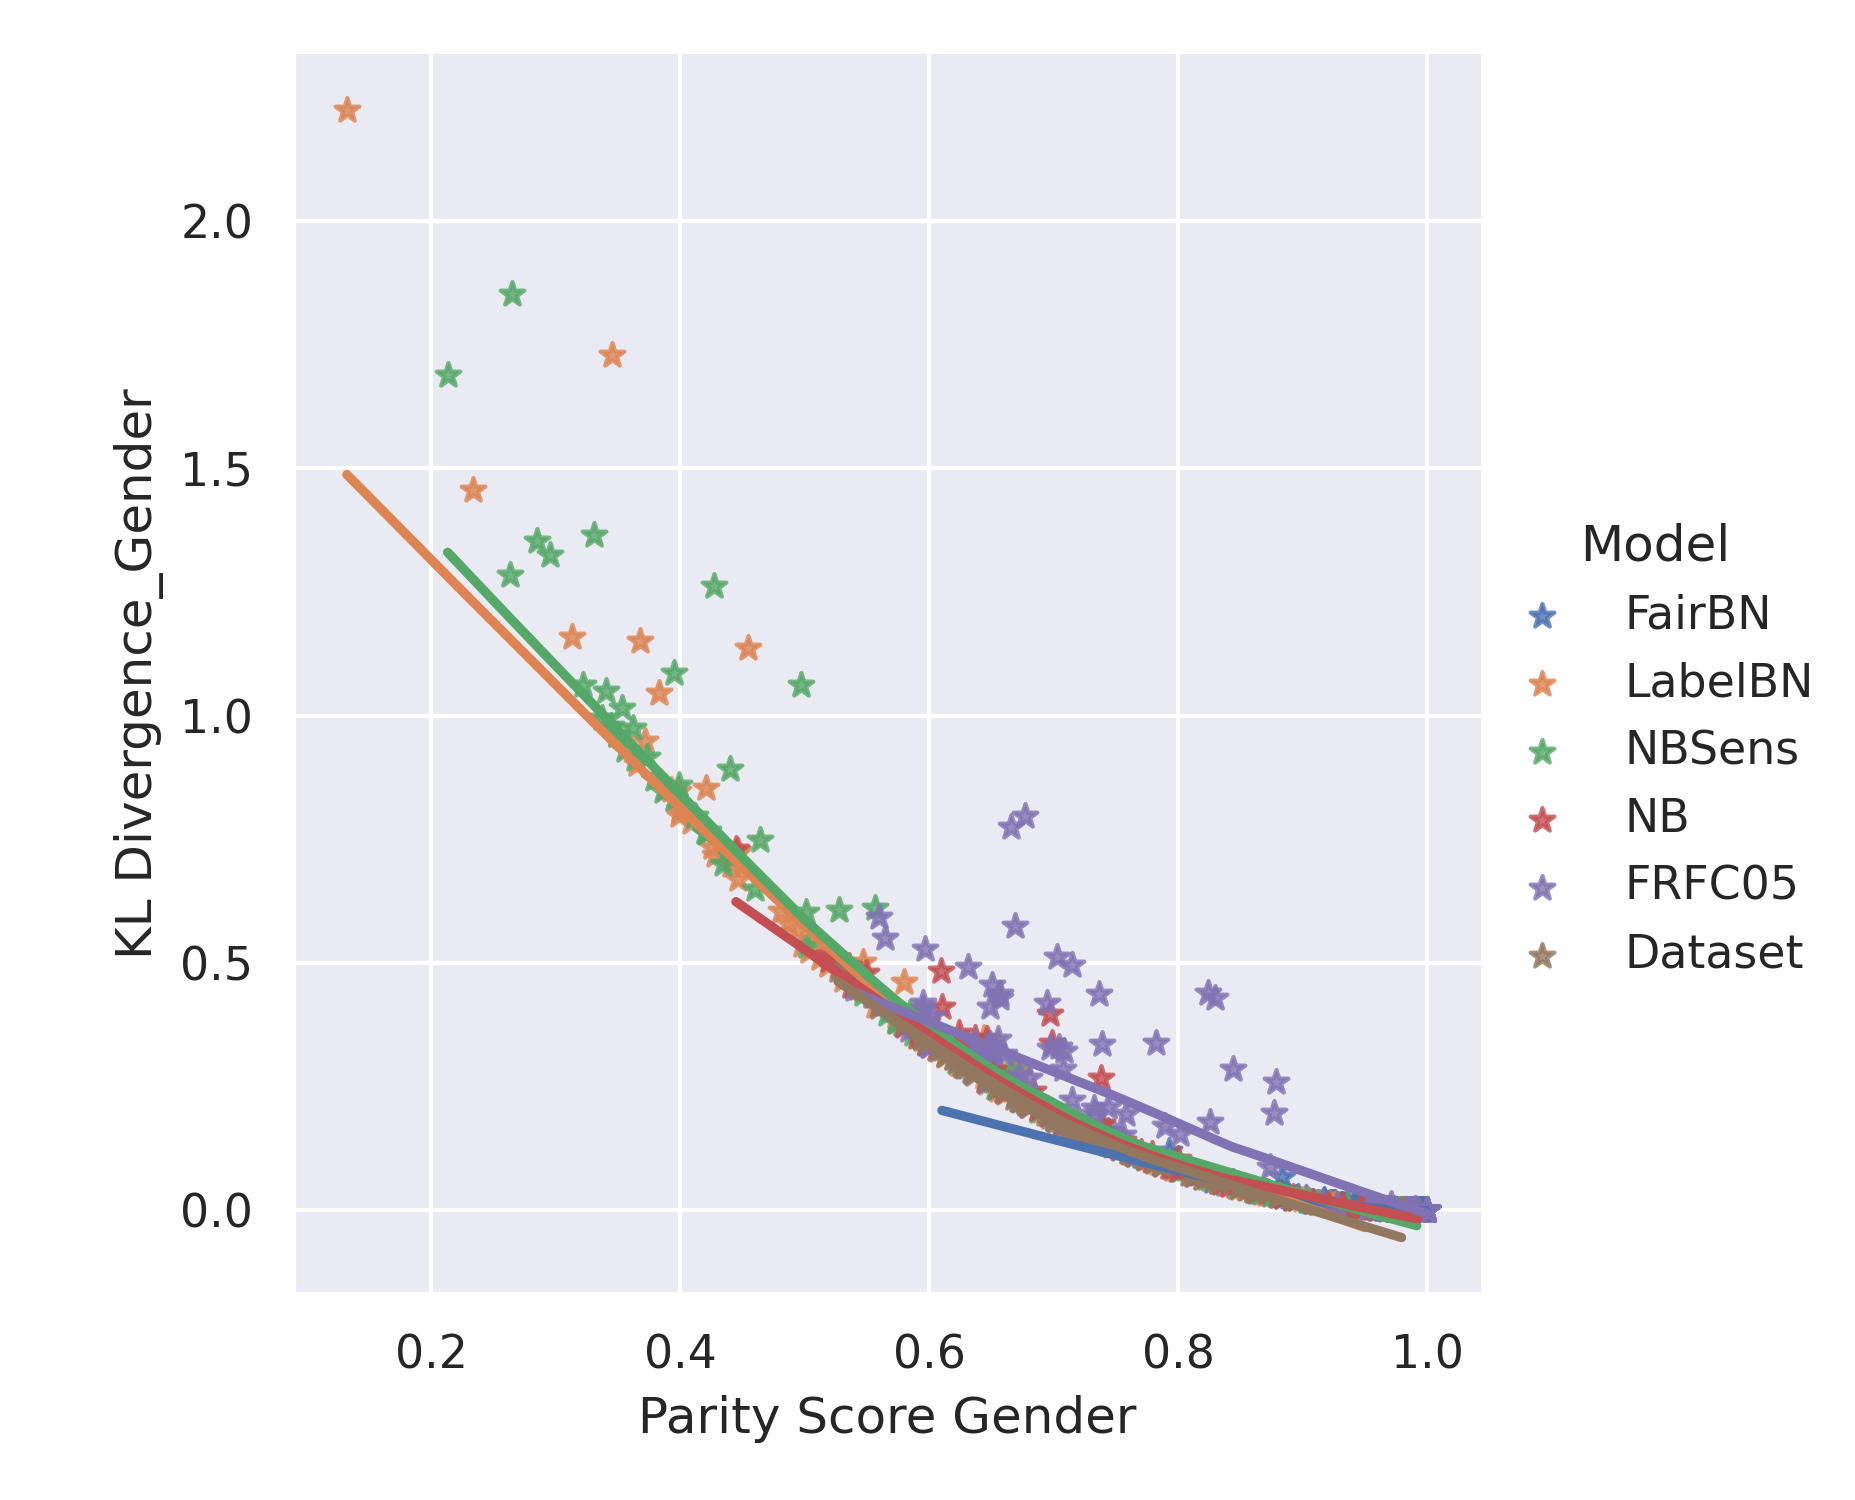
\includegraphics[width=\linewidth]{figures/kldvsdempar-synthethic.png}
    \caption{Demographic Parity and KL Divergence}
    \label{fig:kldvsdempar}
\end{figure}

From figure~\ref{fig:kldvsdempar} we see that demographic parity and KL divergence are inversely related. As the parity score increases the divergence decreases. This gives us further confidence that both measure fairness in terms of demographic parity.

\subsection{AUC and KL Divergence}

\begin{figure}
    \centering
    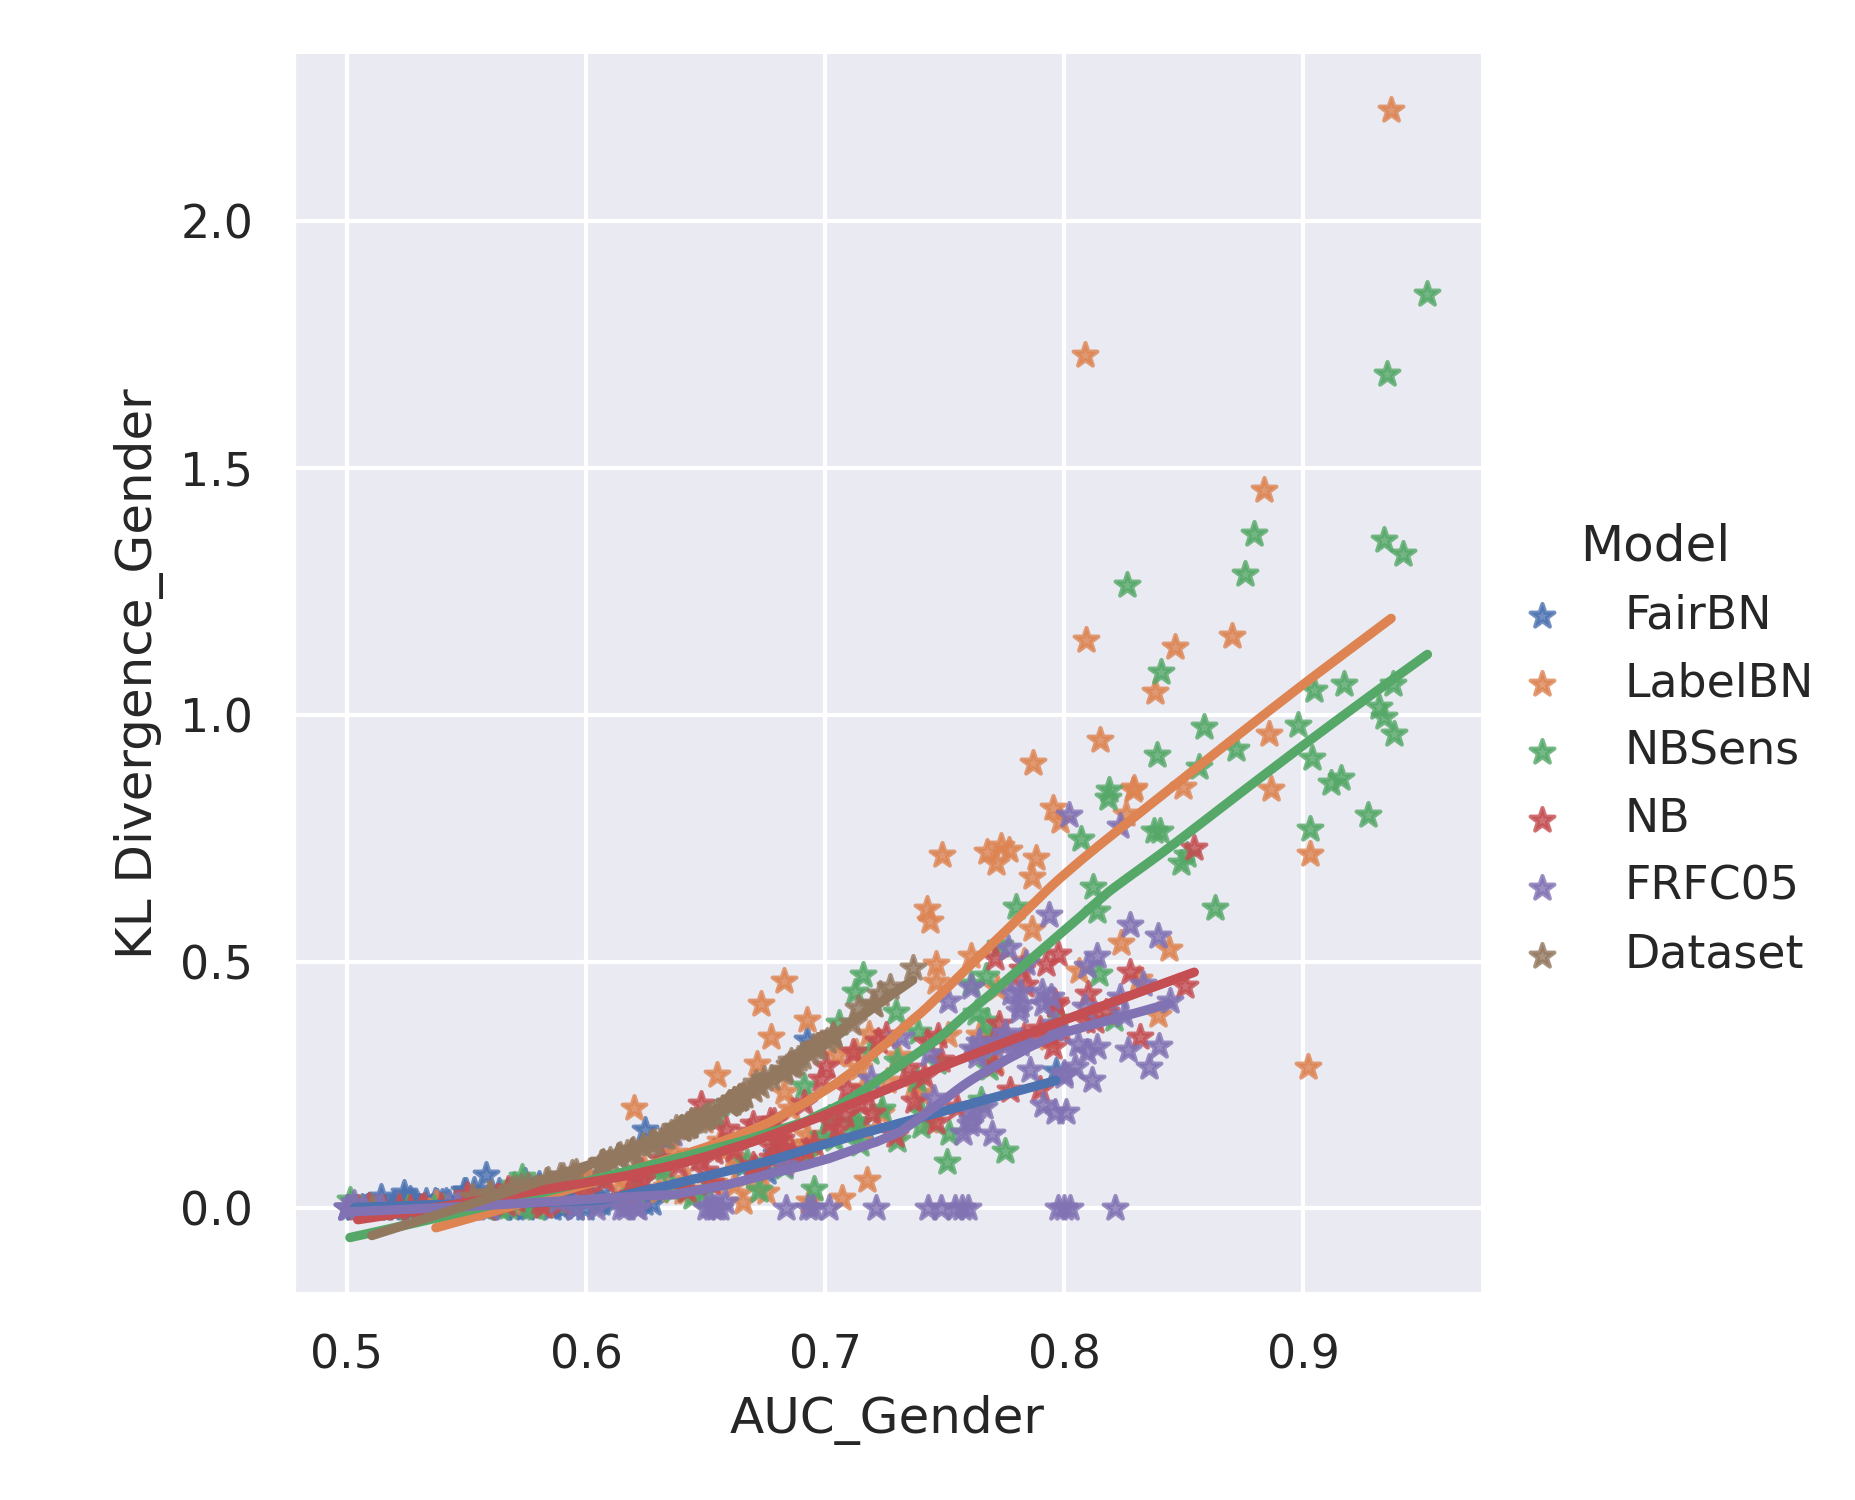
\includegraphics[width=\linewidth]{figures/aucvskldiv-synthethic.png}
    \caption{AUC and KL Divergence w.r.t. Gender}
    \label{fig:aucvskld}
\end{figure}

From figure~\ref{fig:aucvskld} we see that these scores are also correlated with one another, though not as strongly as with Parity Score and KL Divergence. This gives some validity to the use of AUC to train a fair random forest classifier.

\subsection{Hypothesis Tests}

\begin{table}
    \centering
	\begin{tabular}{p{8cm}lll}
        \hline
        \textbf{Hypothesis} & $\boldsymbol{p}$ & Reject $\boldsymbol{H_0}$ & $\boldsymbol{T}$ \\
        \hline
 	    \hline
        FairBN ($Y$) has a better intersectional parity score than naïve Bayes ($X$) without sensitive attributes & $4.13 \times 10^{-18}$ & Yes & $25$ \\ \hline
        FRFC ($Y$) has a better intersectional parity score than naïve Bayes ($X$) without sensitive attributes & $1.93 \times 10^{-9}$ & Yes & $812$ \\ \hline
        FairBN ($Y$) has a better intersectional parity score than FRFC ($X$) & $1.41 \times 10^{-6}$ & Yes & $1163$ \\ \hline
        FairBN ($Y$) has a better KLD w.r.t. Gender than FRFC ($X$) & $2.13 \times 10^{-10}$ & Yes & $4341$ \\ \hline
    \end{tabular}
    \caption{Result of hypothesis tests}
    \label{tab:hypothesisres}
\end{table}

As we see from the table above, we reject the null-hypothesis in all cases. This implies that both fair machine learning models have more fair predictions than the baseline method of using naïve-Bayes without the sensitive attributes. Additionally, we find that the fair Bayesian network has a more consistent and statistically significantly better score than the fair random forest classifier in terms of both parity score and KL Divergence.

\section{Experiment 3: Results}

\subsection{Decision Tree: Adult Dataset}

To gain insight into how the decision tree uses the attributes in its decisions, we calculate the feature importance of all attributes and show the ones that have positive feature importance. Feature importance is calculated as the normalised amount of reduction in entropy brought on by that attribute in the model. After training the decision tree classifier in Scikit-learn on the adult dataset. We got the following feature importance shown in table~\ref{tab:dectreeadultimp}.

\begin{table}[]
    \centering
    \begin{tabular}{lr}
    \toprule
    Attribute &  Importance \\
    \midrule
    marital-status\_Married-civ-spouse &    0.529924 \\
    capital-gain &    0.347748 \\
    education\_Bachelors &    0.041893 \\
    hours-per-week &    0.040666 \\
    age &    0.038778 \\
    education\_Preschool &    0.000992 \\
    \bottomrule
    \end{tabular}
    \caption{Decision Tree: Adult Dataset - Feature Importance}
    \label{tab:dectreeadultimp}
\end{table}

On the adult dataset we see that the decision rules considers whether or not someone has a civilian spouse as the most important variable to consider when classifying someone as high income or not. No sensitive attributes are considered important and when investigating the tree structure, no nodes employ the sensitive attributes.

\subsection{Decision Tree: Compas Dataset}

\begin{table}[]
    \centering
    \begin{tabular}{llr}
    \toprule
    {} &          Attribute &  Importance \\
    \midrule
    0 &       priors\_count &    0.524409 \\
    1 &                age &    0.417728 \\
    2 &           sex\_Male &    0.030951 \\
    3 &     juv\_misd\_count &    0.011672 \\
    4 &  c\_charge\_degree\_M &    0.006723 \\
    5 &         race\_Other &    0.005893 \\
    6 &      juv\_fel\_count &    0.002624 \\
    \bottomrule
    \end{tabular}
    \caption{Decision Tree: Compas Dataset - Feature Importance}
    \label{tab:detreecompasimp}
\end{table}

On the other hand, when training the decision tree classifier on the compas dataset, we see that whether someone is male or considered to belong in the \emph{Other} race category is used in prediction. This implies that there is a significant gender and racial bias in the data.

\subsection{Naive Bayes: Feature Importance}

\begin{figure}
    \centering
    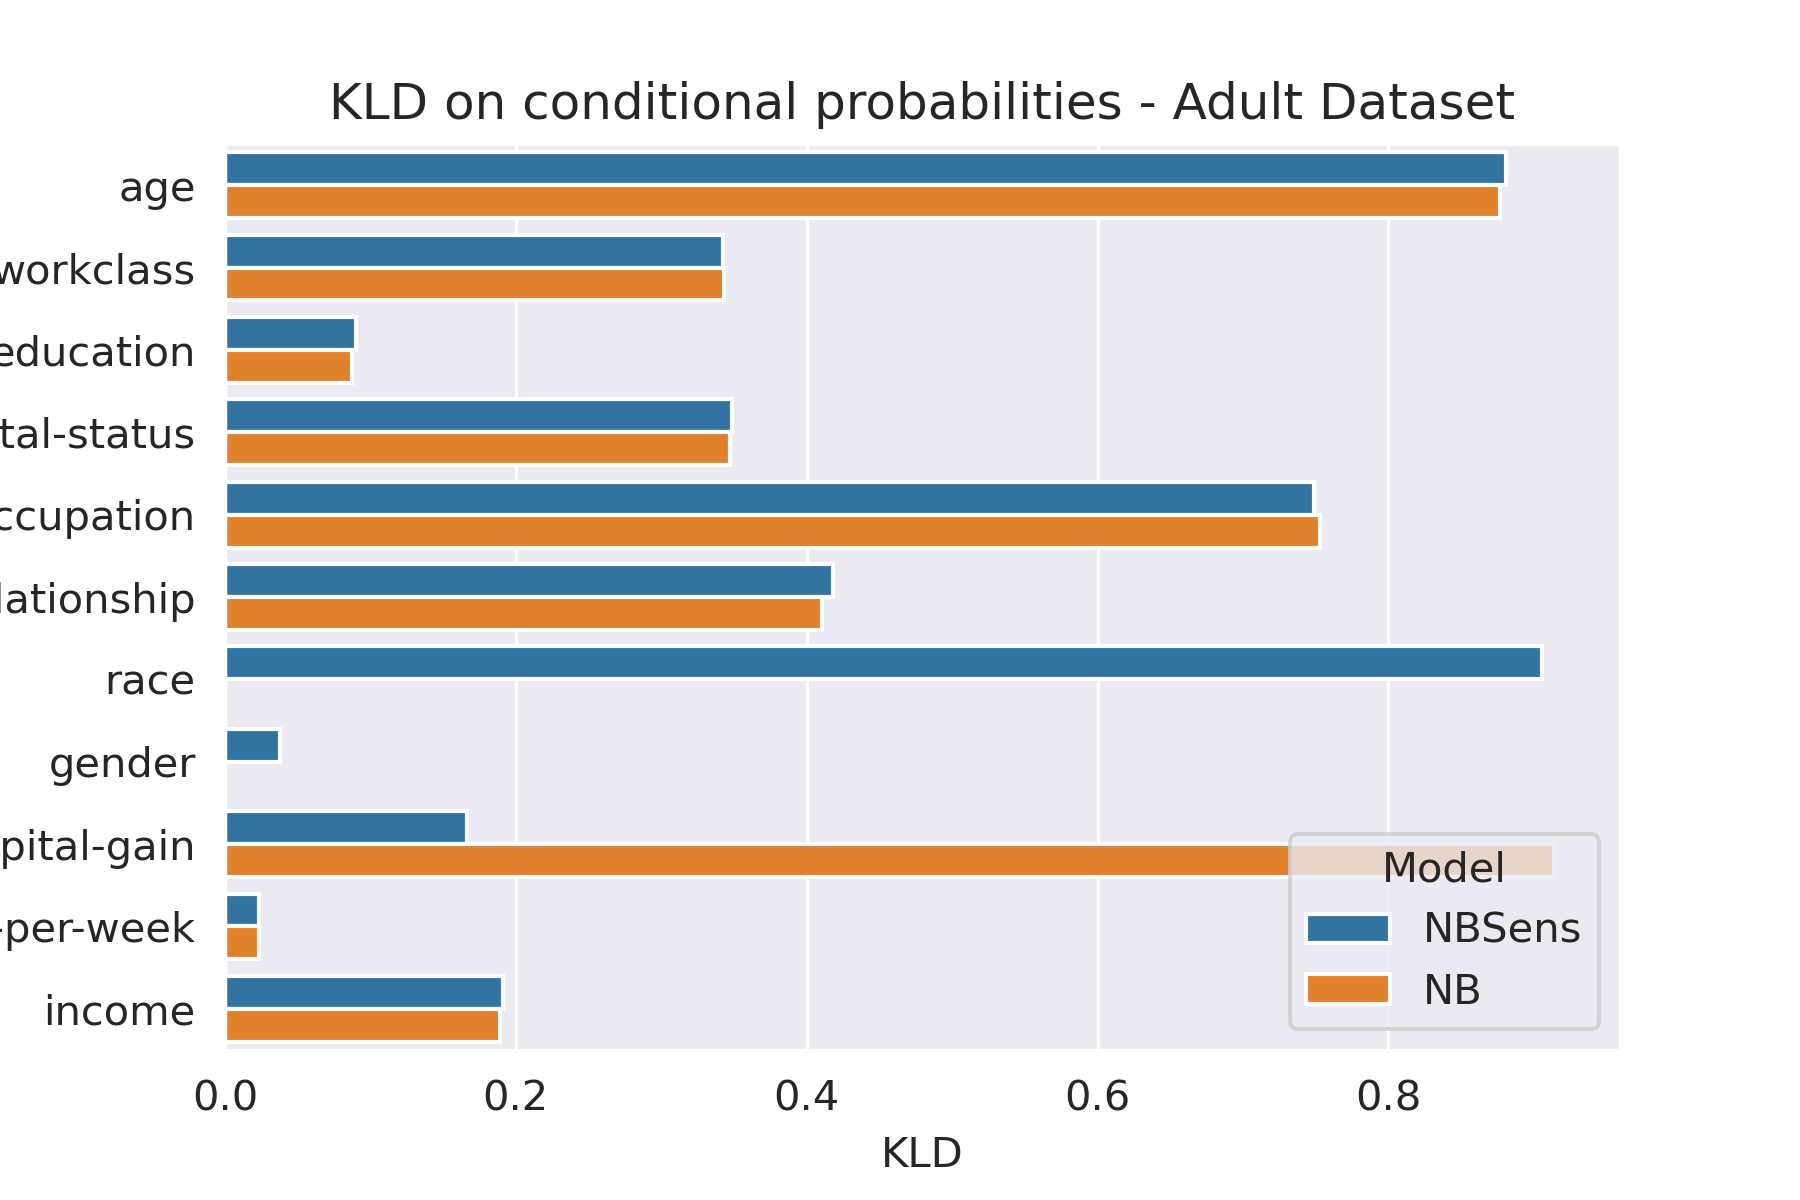
\includegraphics[width=0.49\linewidth]{figures/KLDimportance-adult.png}
    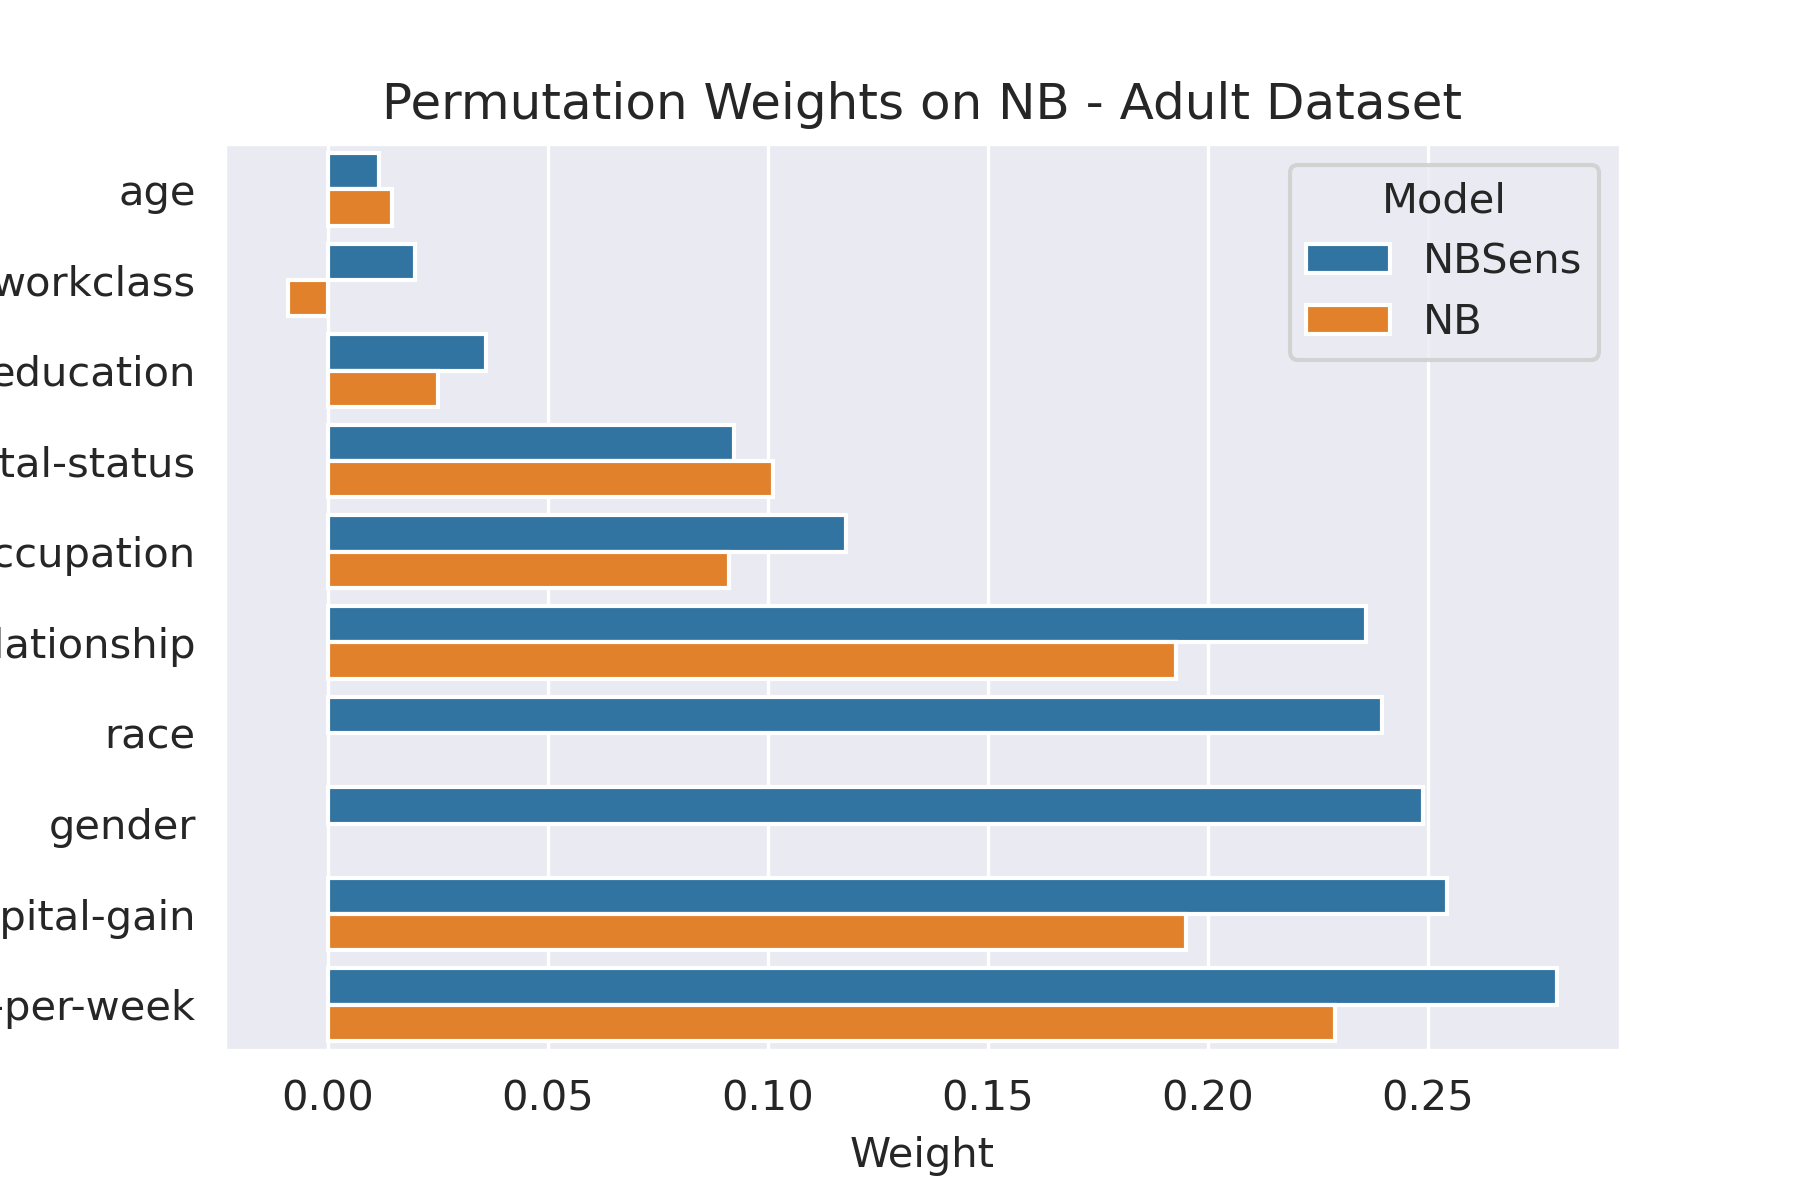
\includegraphics[width=0.49\linewidth]{figures/permimportance-adult.png}
    \caption{KLD and Permutation weights of naïve Bayes with and without sensitive attributes. Adult Dataset.}
    \label{fig:kldpermimpadult}
\end{figure}

To interpret the naïve Bayes models we look at the conditional distributions for the different attributes and compare calculate the KLD between the distribution $P = p(X|Y=0)$ and $Q = p(X|Y=1)$. We also calculate the permutation feature importance by calculating the loss in accuracy by permuting a specific column. The resulting weights are shown in figure~\ref{fig:kldpermimpadult} for the adult datasetn and figure~\ref{fig:kldpermimpcompas}.

\begin{figure}
    \centering
    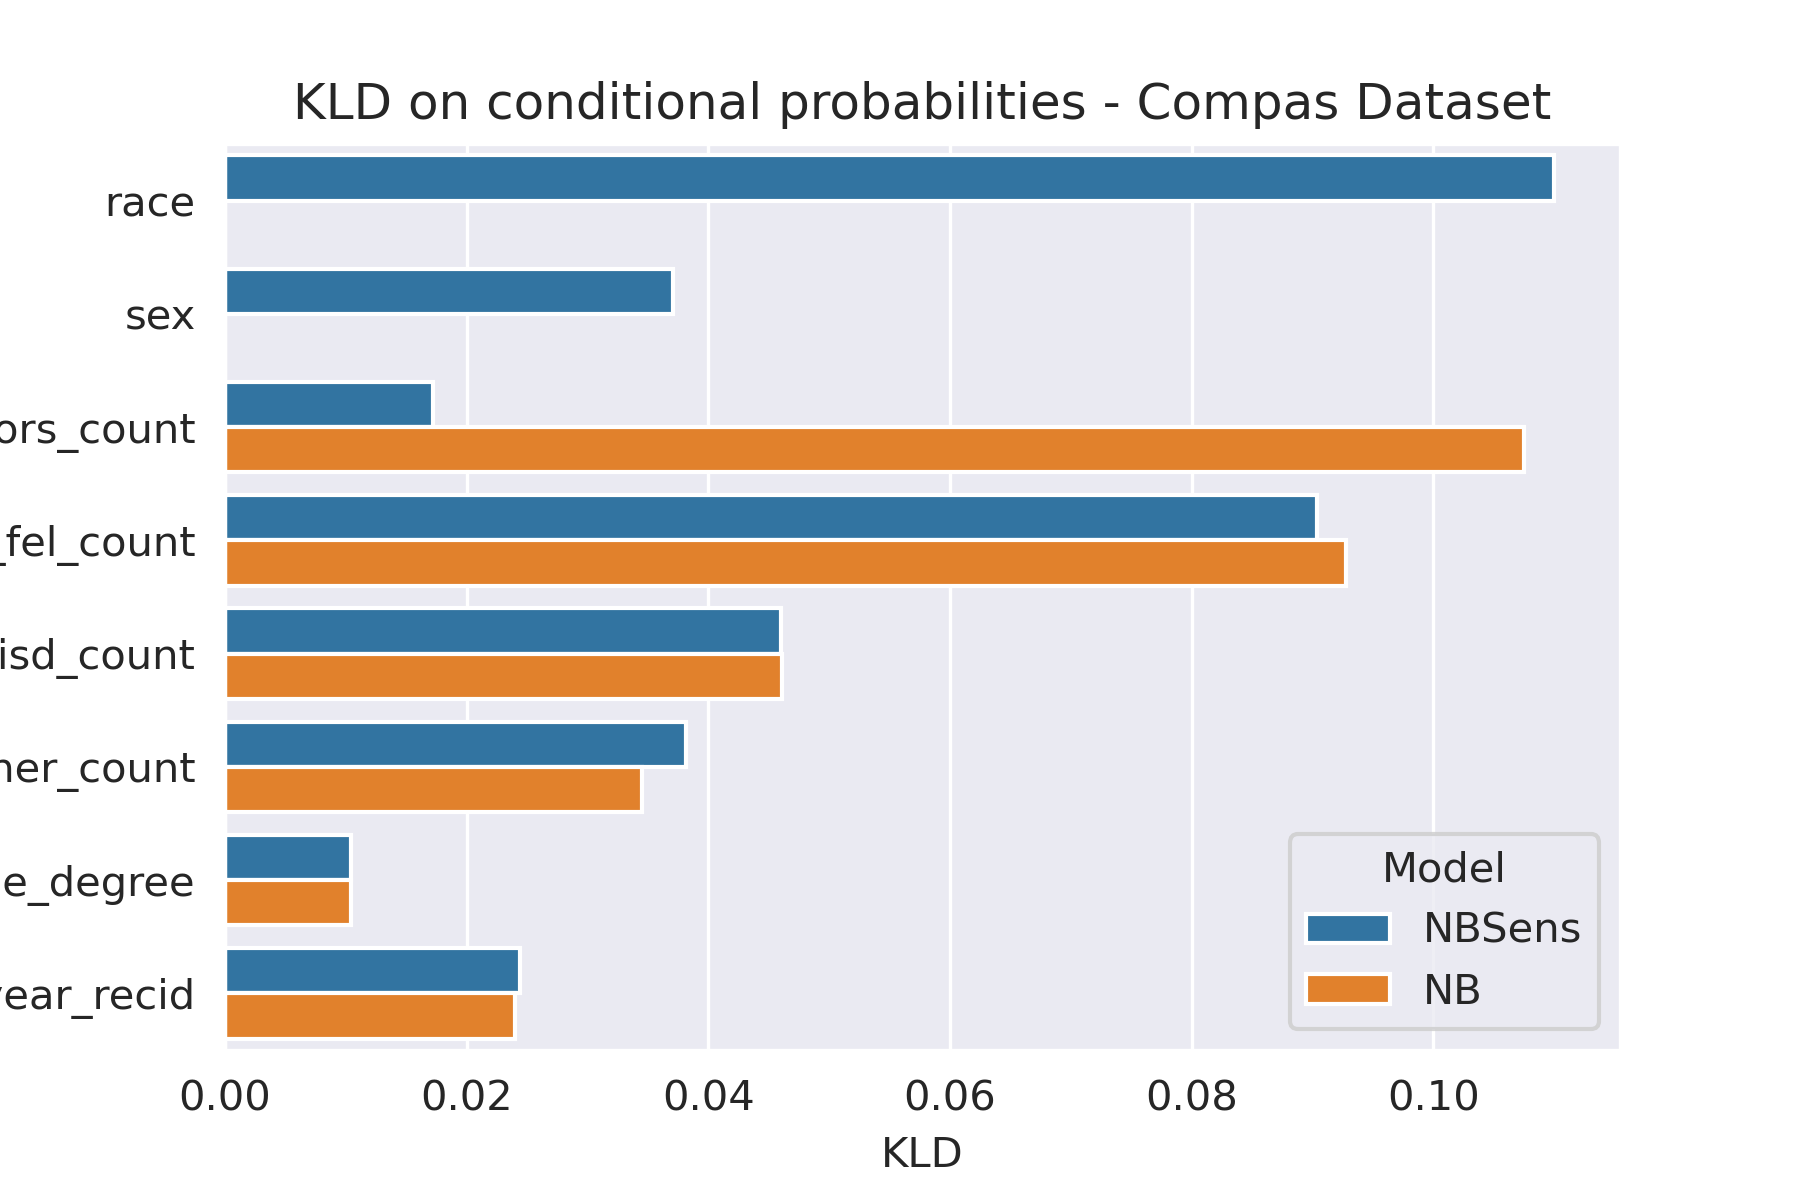
\includegraphics[width=0.49\linewidth]{figures/KLDimportance-compas.png}
    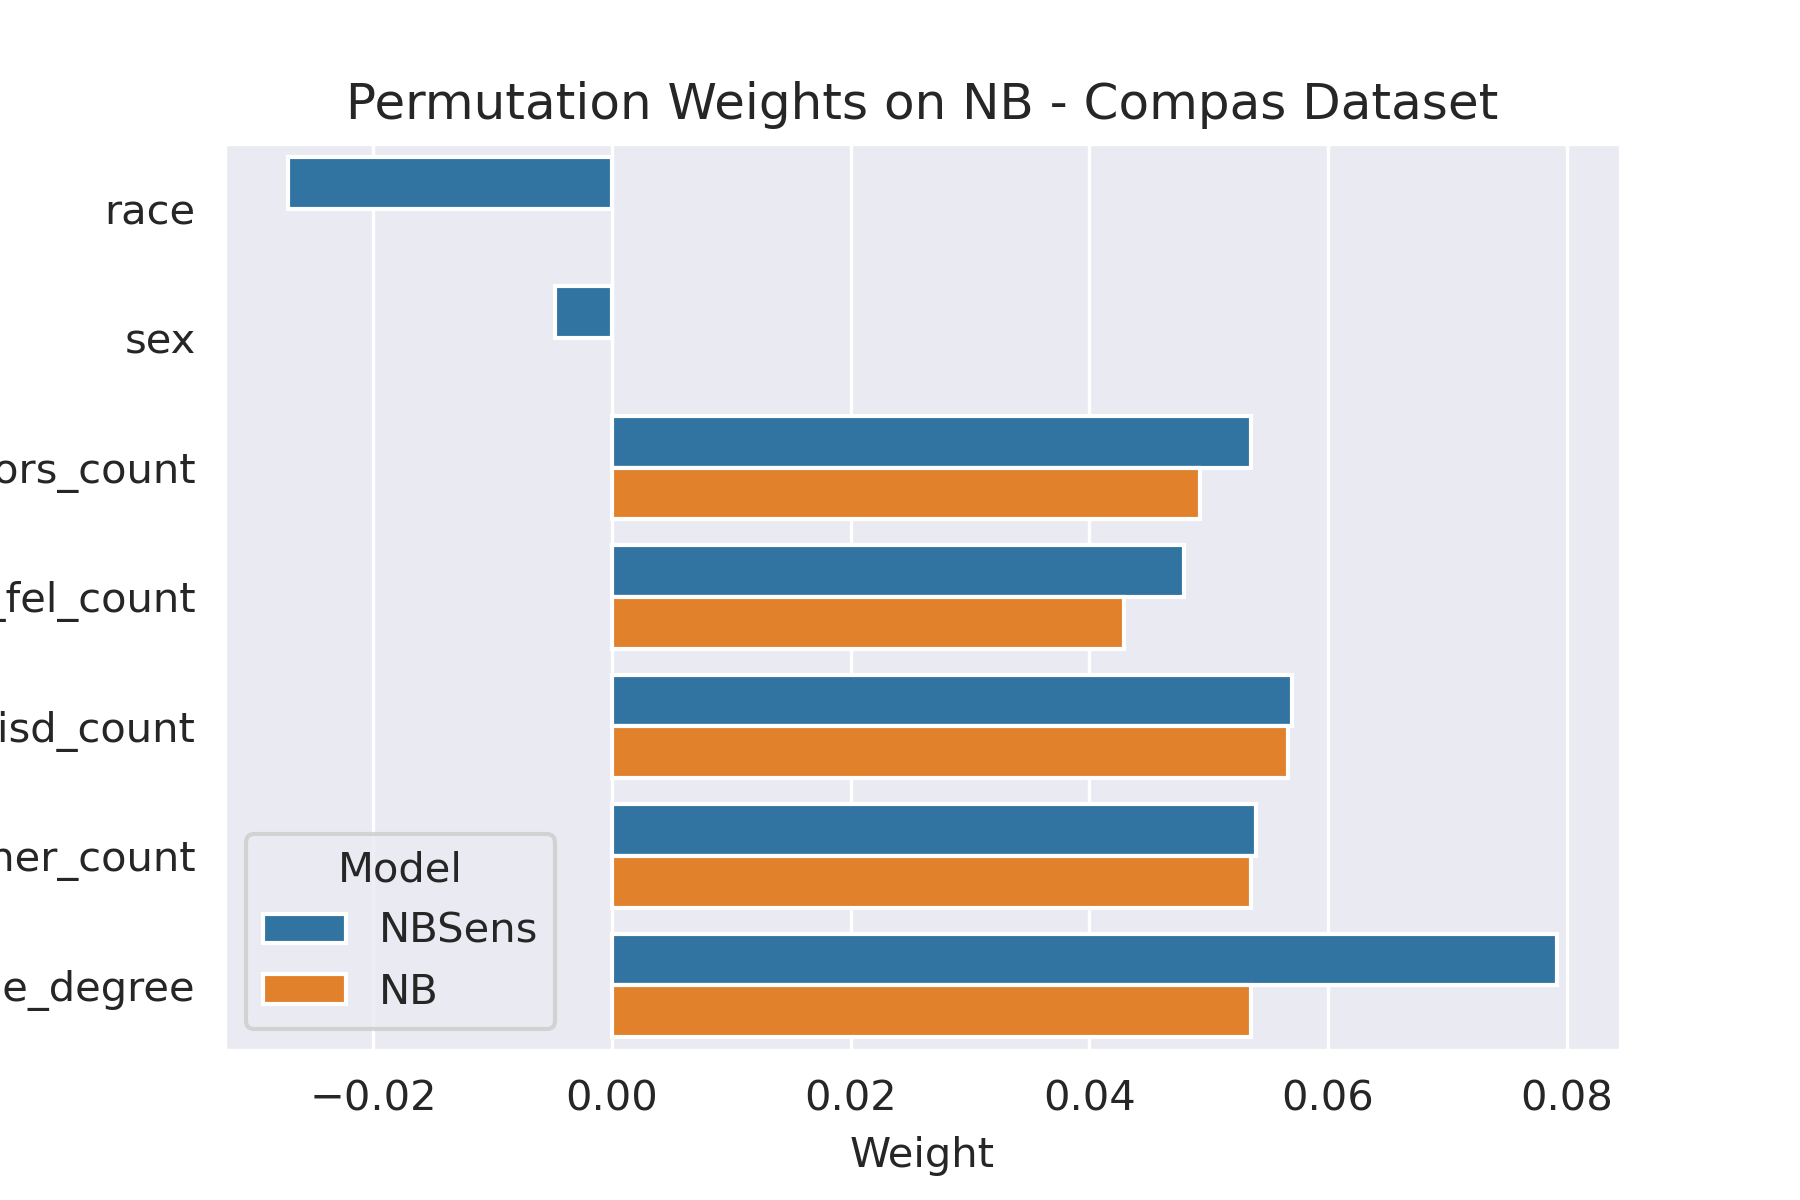
\includegraphics[width=0.49\linewidth]{figures/permimportance-compas.png}
    \caption{KLD and Permutation weights of naïve Bayes with and without sensitive attributes. Compas Dataset.}
    \label{fig:kldpermimpcompas}
\end{figure}

\subsection{Fair Tree Classifier: Feature Importance}

\begin{figure}
    \centering
    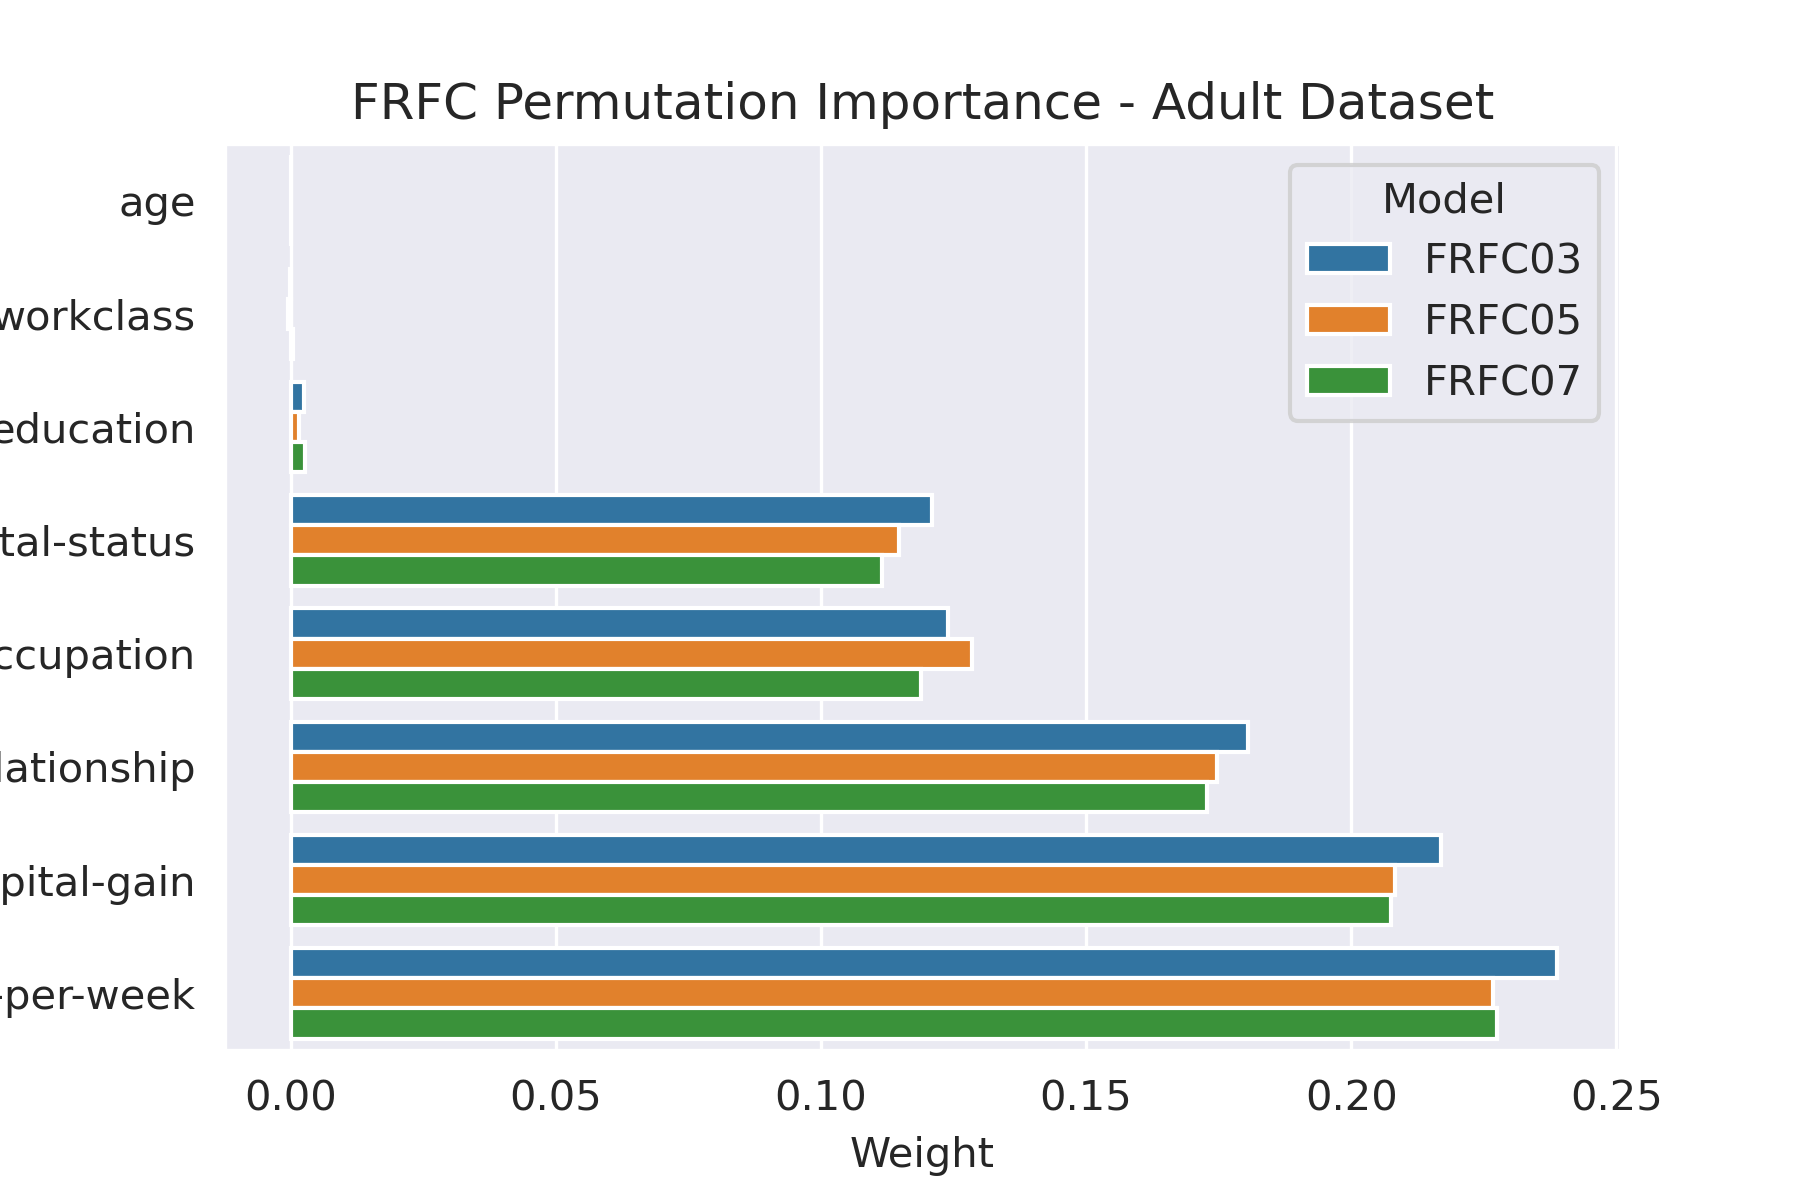
\includegraphics{figures/frfc-permimportance-adult.png}
    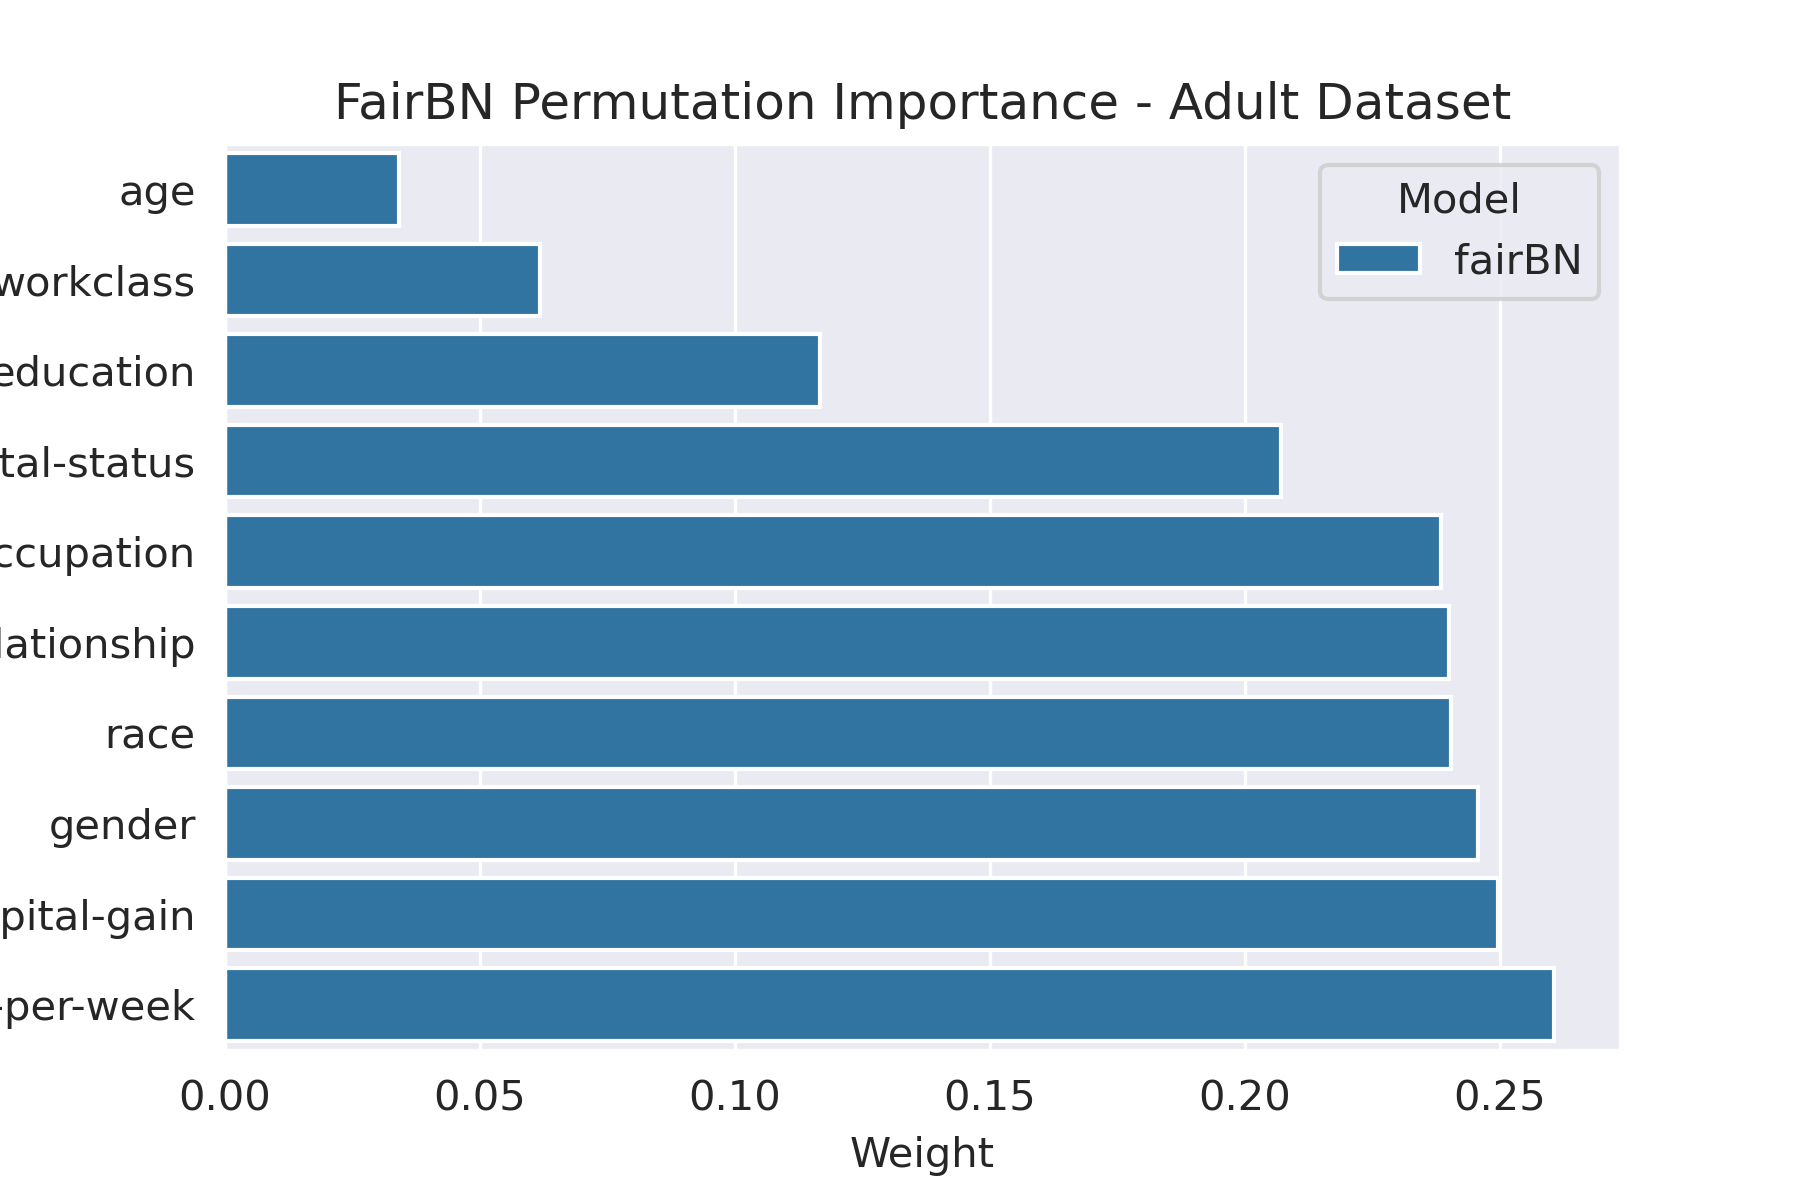
\includegraphics[width=\linewidth]{figures/fairbn-permimportance-adult.png}
    \caption{Caption}
    \label{fig:my_label}
\end{figure}

We also calculate the feature importance of the fair tree classifier. We see a similar relationship in the feature weights as in Naive Bayes but age and work class is completely neglected. Also, as $\Theta$ increases, overall weight of the attributes decreases. 

\subsection{Individual Conditional Expectation}

We have implemented ICE calculations for the classifiers Naive Bayes and Fair Tree Classifiers. As the sensitive attributes are not numerical but categorical, we do not resort to line plots of the predicted probability but rather categorical plots. Therefore, the distribution of predicted probability given the certain values is shown for the different models and datasets. Figure~\ref{fig:ICEdistgenderadult} shows how gender is treated by the different models in the Adult and Compas dataset. Figure~\ref{fig:ICEdistrace} show how race is treated by the different models.

\begin{figure}
    \centering
    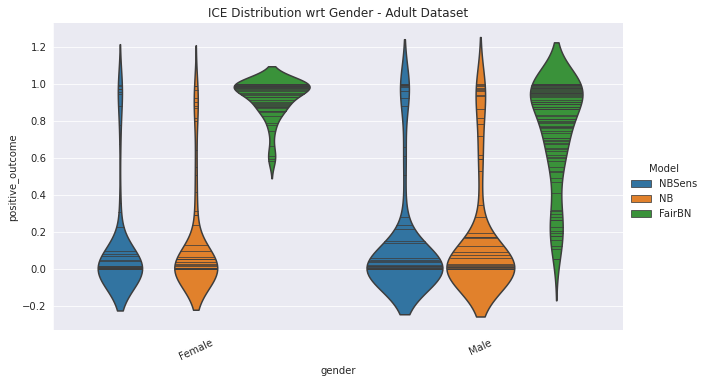
\includegraphics[width=0.49\linewidth]{figures/ICEdistgender-adult.png}
    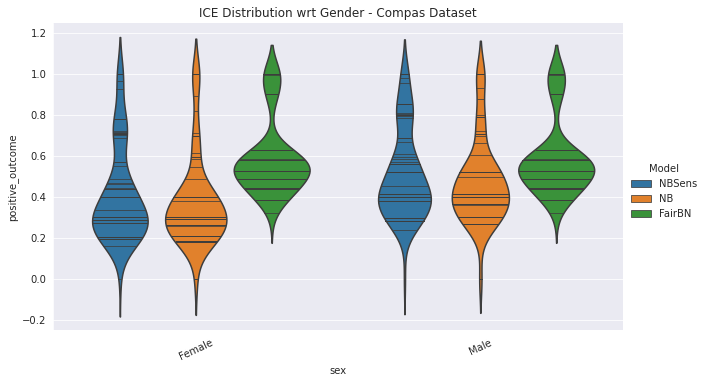
\includegraphics[width=0.49\linewidth]{figures/ICEdistgender-compas.png}
    \caption{ICE distribution for Gender in the different datasets.}
    \label{fig:ICEdistgender}
\end{figure}

\begin{figure}
    \centering
    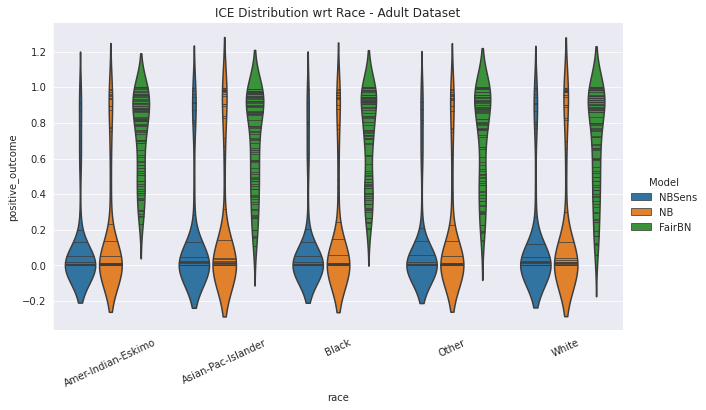
\includegraphics[width=0.49\linewidth]{figures/ICEdistrace-adult.png}
    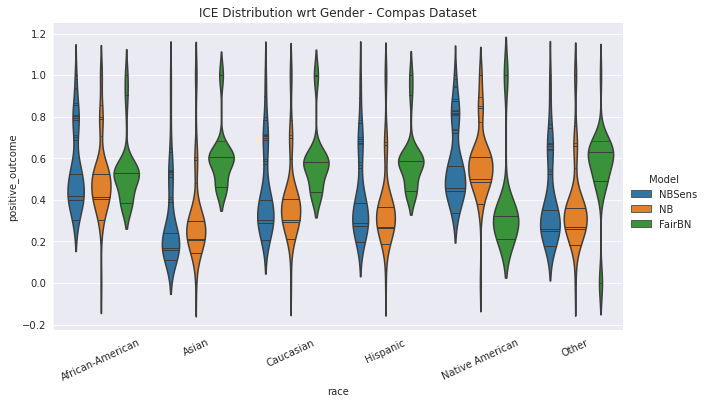
\includegraphics[width=0.49\linewidth]{figures/ICEdistrace-compas.png}
    \caption{ICE distribution for Race in the different datasets}
    \label{fig:ICEdistrace}
\end{figure}


\subsection{Counterfactuals}

\subsubsection{naïve Bayes With Sensitive Attributes}

For the following datapoint:

\resizebox{\textwidth}{!}{
\begin{tabular}{lllllllllll}
\toprule
{} &           age & workclass &  education & marital-status &    occupation & relationship &   race &  gender &          capital-gain & hours-per-week \\
\midrule
46343 &  (31.6, 46.2] &   Private &  Assoc-voc &       Divorced &  Tech-support &    Unmarried &  Black &  Female &  (-4460.355, 16515.0] &   (20.6, 40.2] \\
\bottomrule
\end{tabular}
}

Got the following counterfactuals:

\resizebox{\textwidth}{!}{
\begin{tabular}{lllllllllllrrrr}
\toprule
{} &           age &  workclass &  education &     marital-status &    occupation &   relationship &                race &  gender &        capital-gain & hours-per-week &        O1 &   O2 &  O3 &   O4 \\
\midrule
155 &  (31.6, 46.2] &    Private &  Assoc-voc &  Married-AF-spouse &  Tech-support &      Unmarried &               Black &    Male &  (79128.0, 99999.0] &   (20.6, 40.2] &  0.000000 &  0.7 &   3 &  0.0 \\
162 &  (31.6, 46.2] &    Private &  Assoc-voc &           Divorced &  Adm-clerical &      Unmarried &               Black &    Male &  (79128.0, 99999.0] &   (20.6, 40.2] &  0.000000 &  0.7 &   3 &  0.0 \\
100 &  (31.6, 46.2] &    Private &  Assoc-voc &  Married-AF-spouse &  Adm-clerical &      Unmarried &               Black &    Male &  (58257.0, 79128.0] &   (20.6, 40.2] &  0.000000 &  0.6 &   4 &  0.0 \\
167 &  (31.6, 46.2] &    Private &  Assoc-voc &  Married-AF-spouse &  Adm-clerical &      Unmarried &               Black &    Male &  (79128.0, 99999.0] &   (20.6, 40.2] &  0.000000 &  0.6 &   4 &  0.0 \\
176 &  (31.6, 46.2] &    Private &  Assoc-voc &  Married-AF-spouse &  Adm-clerical &      Unmarried &               Black &    Male &  (58257.0, 79128.0] &   (20.6, 40.2] &  0.000000 &  0.6 &   4 &  0.0 \\
2   &  (60.8, 75.4] &  Local-gov &  Doctorate &           Divorced &             ? &  Not-in-family &  Amer-Indian-Eskimo &  Female &  (79128.0, 99999.0] &   (59.8, 79.4] &  0.000000 &  0.2 &   8 &  0.0 \\
177 &  (31.6, 46.2] &    Private &  Assoc-voc &  Married-AF-spouse &  Tech-support &      Unmarried &               Black &  Female &  (16515.0, 37386.0] &   (20.6, 40.2] &  0.419303 &  0.8 &   2 &  0.0 \\
\bottomrule
\end{tabular}
}

\subsubsection{naïve Bayes Without Sensitive Attributes}

For the following datapoint:

\resizebox{\textwidth}{!}{
\begin{tabular}{lllllllllll}
\toprule
{} &             age & workclass & education & marital-status & occupation & relationship &   race &  gender &          capital-gain & hours-per-week \\
\midrule
23356 &  (16.927, 31.6] &         ? &   HS-grad &      Separated &          ? &    Unmarried &  Black &  Female &  (-4460.355, 16515.0] &   (20.6, 40.2] \\
\bottomrule
\end{tabular}
} 

We get the following counterfactuals:

\resizebox{\textwidth}{!}{
\begin{tabular}{lllllllllllrrrr}
\toprule
{} &             age &  workclass &  education &     marital-status & occupation &   relationship &                race &  gender &          capital-gain & hours-per-week &        O1 &   O2 &  O3 &   O4 \\
\midrule
128 &  (16.927, 31.6] &  State-gov &    HS-grad &          Separated &          ? &      Unmarried &               Black &    Male &    (79128.0, 99999.0] &   (20.6, 40.2] &  0.000000 &  0.7 &   3 &  0.0 \\
97  &    (31.6, 46.2] &          ? &    HS-grad &          Separated &          ? &  Not-in-family &               Black &    Male &    (79128.0, 99999.0] &   (20.6, 40.2] &  0.000000 &  0.6 &   4 &  0.0 \\
147 &  (16.927, 31.6] &  State-gov &  Doctorate &          Separated &          ? &      Unmarried &               Black &    Male &    (79128.0, 99999.0] &   (20.6, 40.2] &  0.000000 &  0.6 &   4 &  0.0 \\
136 &    (31.6, 46.2] &  State-gov &  Doctorate &  Married-AF-spouse &          ? &        Husband &  Amer-Indian-Eskimo &  Female &  (-4460.355, 16515.0] &   (20.6, 40.2] &  0.165877 &  0.4 &   6 &  0.1 \\
\bottomrule
\end{tabular}
}

\subsubsection{Fair Bayesian Network}

For the following counterfactual

\resizebox{\textwidth}{!}{
\begin{tabular}{lllllllllll}
\toprule
{} &             age & workclass & education & marital-status & occupation & relationship &   race &  gender &          capital-gain & hours-per-week \\
\midrule
23356 &  (16.927, 31.6] &         ? &   HS-grad &      Separated &          ? &    Unmarried &  Black &  Female &  (-4460.355, 16515.0] &   (20.6, 40.2] \\
\bottomrule
\end{tabular}
}

We get the following counterfactuals

\resizebox{\textwidth}{!}{
\begin{tabular}{lllllllllllrrrr}
\toprule
{} &             age &         workclass &   education & marital-status &       occupation &   relationship &                race &  gender &        capital-gain & hours-per-week &            O1 &   O2 &  O3 &   O4 \\
\midrule
111 &  (16.927, 31.6] &                 ? &        11th &      Separated &                ? &      Unmarried &               Black &  Female &  (79128.0, 99999.0] &   (79.4, 99.0] &  0.000000e+00 &  0.7 &   3 &  0.0 \\
114 &  (16.927, 31.6] &                 ? &     HS-grad &      Separated &                ? &      Unmarried &               White &  Female &  (79128.0, 99999.0] &   (79.4, 99.0] &  0.000000e+00 &  0.7 &   3 &  0.0 \\
162 &  (16.927, 31.6] &                 ? &        11th &      Separated &                ? &      Unmarried &               White &  Female &  (79128.0, 99999.0] &   (20.6, 40.2] &  0.000000e+00 &  0.7 &   3 &  0.1 \\
58  &  (16.927, 31.6] &      Never-worked &     HS-grad &      Separated &                ? &      Unmarried &  Asian-Pac-Islander &  Female &  (58257.0, 79128.0] &   (79.4, 99.0] &  0.000000e+00 &  0.6 &   4 &  0.0 \\
118 &  (16.927, 31.6] &                 ? &  Assoc-acdm &      Separated &                ? &      Unmarried &               Black &    Male &  (79128.0, 99999.0] &   (79.4, 99.0] &  0.000000e+00 &  0.6 &   4 &  0.0 \\
172 &  (16.927, 31.6] &      Never-worked &        11th &      Separated &                ? &      Unmarried &               White &  Female &  (58257.0, 79128.0] &   (20.6, 40.2] &  0.000000e+00 &  0.6 &   4 &  0.1 \\
\end{tabular}
}